% !TEX encoding = UTF-8
% !TEX TS-program = pdflatex
% !TEX root = ../tesi.tex

%**************************************************************
\chapter{Realizzazione}
\label{cap:realizzazione}
%**************************************************************



\section{Studio delle tecnologie}
\subsection{Flutter}
E' impossibile parlare di Flutter senza prima discutere del linguaggio su cui si basa: Dart.\\
Faremo quindi un'introduzione quanto più sintetica possibile sulle sue caratteristiche più proprietarie, tralasciando invece le similitudini a linguaggi popolari che possono facilmente essere intuite dal lettore.
\subsubsection{Dart}
Dart è un linguaggio compilato fortemente tipizzato con sintassi simile a C, e adotta molte funzionalità tipiche dei linguaggi moderni: considera infatti ogni variabile un oggetto e implementa la \textit{null safety}, obbligando il programmatore a esplicitare con sintassi specifiche la presenza o meno del valore \verb+null+.

\begin{lstlisting}[language=dart, firstnumber=1,caption={Dart \textit{null safety}}]
    //dichiarazione di variabili
    String variabileNotNullable = '';  //non puo' mai essere null
    String? variabileNullable = null;  //puo' anche essere null

    //utilizzo esplicito di variabile nullable
    fun (variableNullable);   //compile error
    fun (?variableNullable);  //esplicito che puo' essere nulla

    //utilizzo esplicito di variabile not nullable
    if (value != null)
        fun (!value);   //dico al compilatore che sono certo value non sia null
\end{lstlisting} 

Permette inoltre l'interpolazione di stringhe:

\begin{lstlisting}[language=dart, firstnumber=1,caption={Dart interpolazone stringhe}]
    //sfrutto il simbolo $
    'number = $variableName';              //inserisco in stringa direttamente una variabile
    'expressionResult = ${expression}';    //inserisco in stringa direttamente un'espressione
\end{lstlisting}

Dart tratta in maniera particolare le funzioni, che sono oggetti, hanno un tipo (\verb+Function+), possono avere parametri posizioni o nominali, obbligatori od opzionali: 

\begin{lstlisting}[language=dart, firstnumber=1,caption={Dart parametri funzioni}]
    //parametri obbligatori posizionali
    void fun (int a, int b);  //non possono essere nulli, non essendo 'int? a'

    //possono essere anteceduti da parametri posizionali opzionali
    void fun (int a, int b, [String opz1 = '', String opz2 = '']){}
    void fun (int a, int b, [String? opz1nullable, String? opz2nullable]){}

    //oppure possono essere anteceduti da parametri nominali opzionali
    void fun (int a, int b, {String opz1 = '', String opz2 = ''}){}
    void fun (int a, int b, {String? opz1nullable, String? opz2nullable}){}

    //non possono essere anteceduti da entrambi
    void fun (int a, int b, [String opz1 = ''], {String opz2 = ''}){} //compile error

    //tutti i costruttori in Dart hanno solo parametri nominali
    //di default i parametri nominali sono opzionali
    //possono pero' essere resi obbligatori con la keyword 'required'
    void fun ({required String obb1, required String? obb2, String opz1 = ''}){}
\end{lstlisting}

Esistono le funzioni anonime (largamente sfruttate nei metodi \verb+build+ di Flutter), che possono essere ovviamente passate come argomento ad altre funzioni, essendo oggetti:

\begin{lstlisting}[language=dart, firstnumber=1,caption={Dart funzioni anonime}]
    //prima sintassi
    (){
        //corpo della funzione anonima
    } 

    //seconda sintassi
    () => return_expression

    //assegnamento di funzione anonima ad una variabile
    //ritorna una stringa con un messaggio portato in upper case
    var upperfy = (msg) => '${msg.toUpperCase()}';

    //passaggio di funzione come parametro
    fun (firstValue, () => secondValue);
\end{lstlisting}

Abbiamo delle espressioni condizionali specifiche del linguaggio dalla grande espressività e che quindi vengono largamente usate:

\begin{lstlisting}[language=dart, firstnumber=1,caption={Dart espressioni ternarie}]
    //primo tipo di condizione, detta ternaria
    condizione ? expr1 : expr2;

    //equivale a (in pseudocodice):
    if (condizione == true) return expr1
    else                    return expr2

    //vediamo un esempio
    int? a;               //a==null di default
    a = a==null ? 1 : 0;  //ad 'a' viene assegnato il valore 1 siccome a==null


    //################################
    //secondo tipo di condizione peculiare:
    expr1 ?? expr2;

    //equivale a (in pseudocodice):
    if (expr1 != null) return expr1
    else               return expr2

    //vediamo un esempio
    int? a;      //a==null di default
    a = a ?? 1;  //ad 'a' viene assegnato il valore 1 siccome a==null
\end{lstlisting}

I caratteri \verb+?+ e \verb+!+ sono, come si evince dalle espressioni ternarie e dalla \textit{null safety}, di cruciale importanza in Dart, ed è quindi opportuno vedere ancora qualche esempio del loro utilizzo:

\begin{lstlisting}[language=dart, firstnumber=1,caption={Dart operatori '?' e '!'}]
    list[1]     //accede al secondo elemento della lista

    list.?[1]
    //equivale a (in pseudocodice):
    if (list[1] != null)    return list[1]
    else                    return null

    //##############################

    foo?.bar 
    //equivale a (in pseudocodice):
    if (foo.bar != null)    return foo.bar
    else                    return null

    //##############################

    foo!.bar
    //equivale a (in pseudocodice):
    if (foo.bar != null)    return foo.bar
    else                    throw (runtimeException)
\end{lstlisting}

Le applicazioni \textit{mobile} e \textit{web} spesso si trovano a eseguire istruzioni che richiedono l'attesa di risorse esterne (ottenere dati dalla rete o leggerli da un \textit{file}, oppure scrivere su un \textit{database}). Per evitare il completo blocco dell'esecuzione (disastroso per un applicativo \textit{consumer}) Dart implementa nativamente delle funzioni di programmazione asincrona, che permetto di svolgere operazioni anche mentre altre sono in attesa.\\
Per fare ciò si serve di tre \textit{keyword}: \verb+async+, \verb+await+ e \verb+Future+:

\begin{lstlisting}[language=dart, firstnumber=1,caption={Dart programmazione asincrona}]
    Future<void> checkVersion () async {
        var version = await lookUpVersion();
    }

    //un'espressione marcata con la keyword 'await' ritorna sempre Future<T>
\end{lstlisting}

Trattiamo infine le caratteristiche peculiari di Dart per quanto riguarda classi e metodi:

\begin{itemize}
    \item Esistono i costruttori costanti, marcati \verb+const+, che sono inizializzati a \textit{compile-time}. Tutti gli altri sono implicitamente dinamici (quindi \textit{run-time});
    \item Posso creare costruttori nominati per implementare costruttori multipli tramite la sintassi:
\begin{lstlisting}[language=dart]
    ClassName.constructorName () :
        firstField = firstValue,
        secondField = secondValue;
\end{lstlisting}
    \item Ogni entità è una classe, ogni classe discende da \verb+Object+ (ad eccezione di \verb+Null+);
    \item Per ogni classe viene creata un'interfaccia implicita che contiene tutti i membri di istanza della classe;
    \item I metodi \textit{getter} e \textit{setter} di una classe vengono creati implicitamente per variabili non \verb+final+, ma possono essere definiti esplicitamente con le \textit{keyword} \verb+get+ e \verb+set+.
\end{itemize}

\subsubsection{Widget}
Mostriamo ora alcuni componenti di Flutter necessari al proseguimento della lettura, partendo dai \textit{widget}: riprendono l'idea di React di costruire tutta l'interfaccia grafica tramite uno \textit{stack} di \textit{widget}, che definiscono il proprio aspetto basandosi sulla configurazione e lo stato attuali. Quando lo stato di un \textit{widget} cambia, esso riscrive la propria descrizione (insieme di istruzioni e valori che lo determinano) e il \textit{framework} valuta le differenze tra questa e la descrizione precedente per apportare le modifiche necessarie al suo \textit{render tree} e quindi, ultimamente, modificarne l'aspetto e finalizzare il cambio di stato.

\begin{figure}[H]
    \centering
    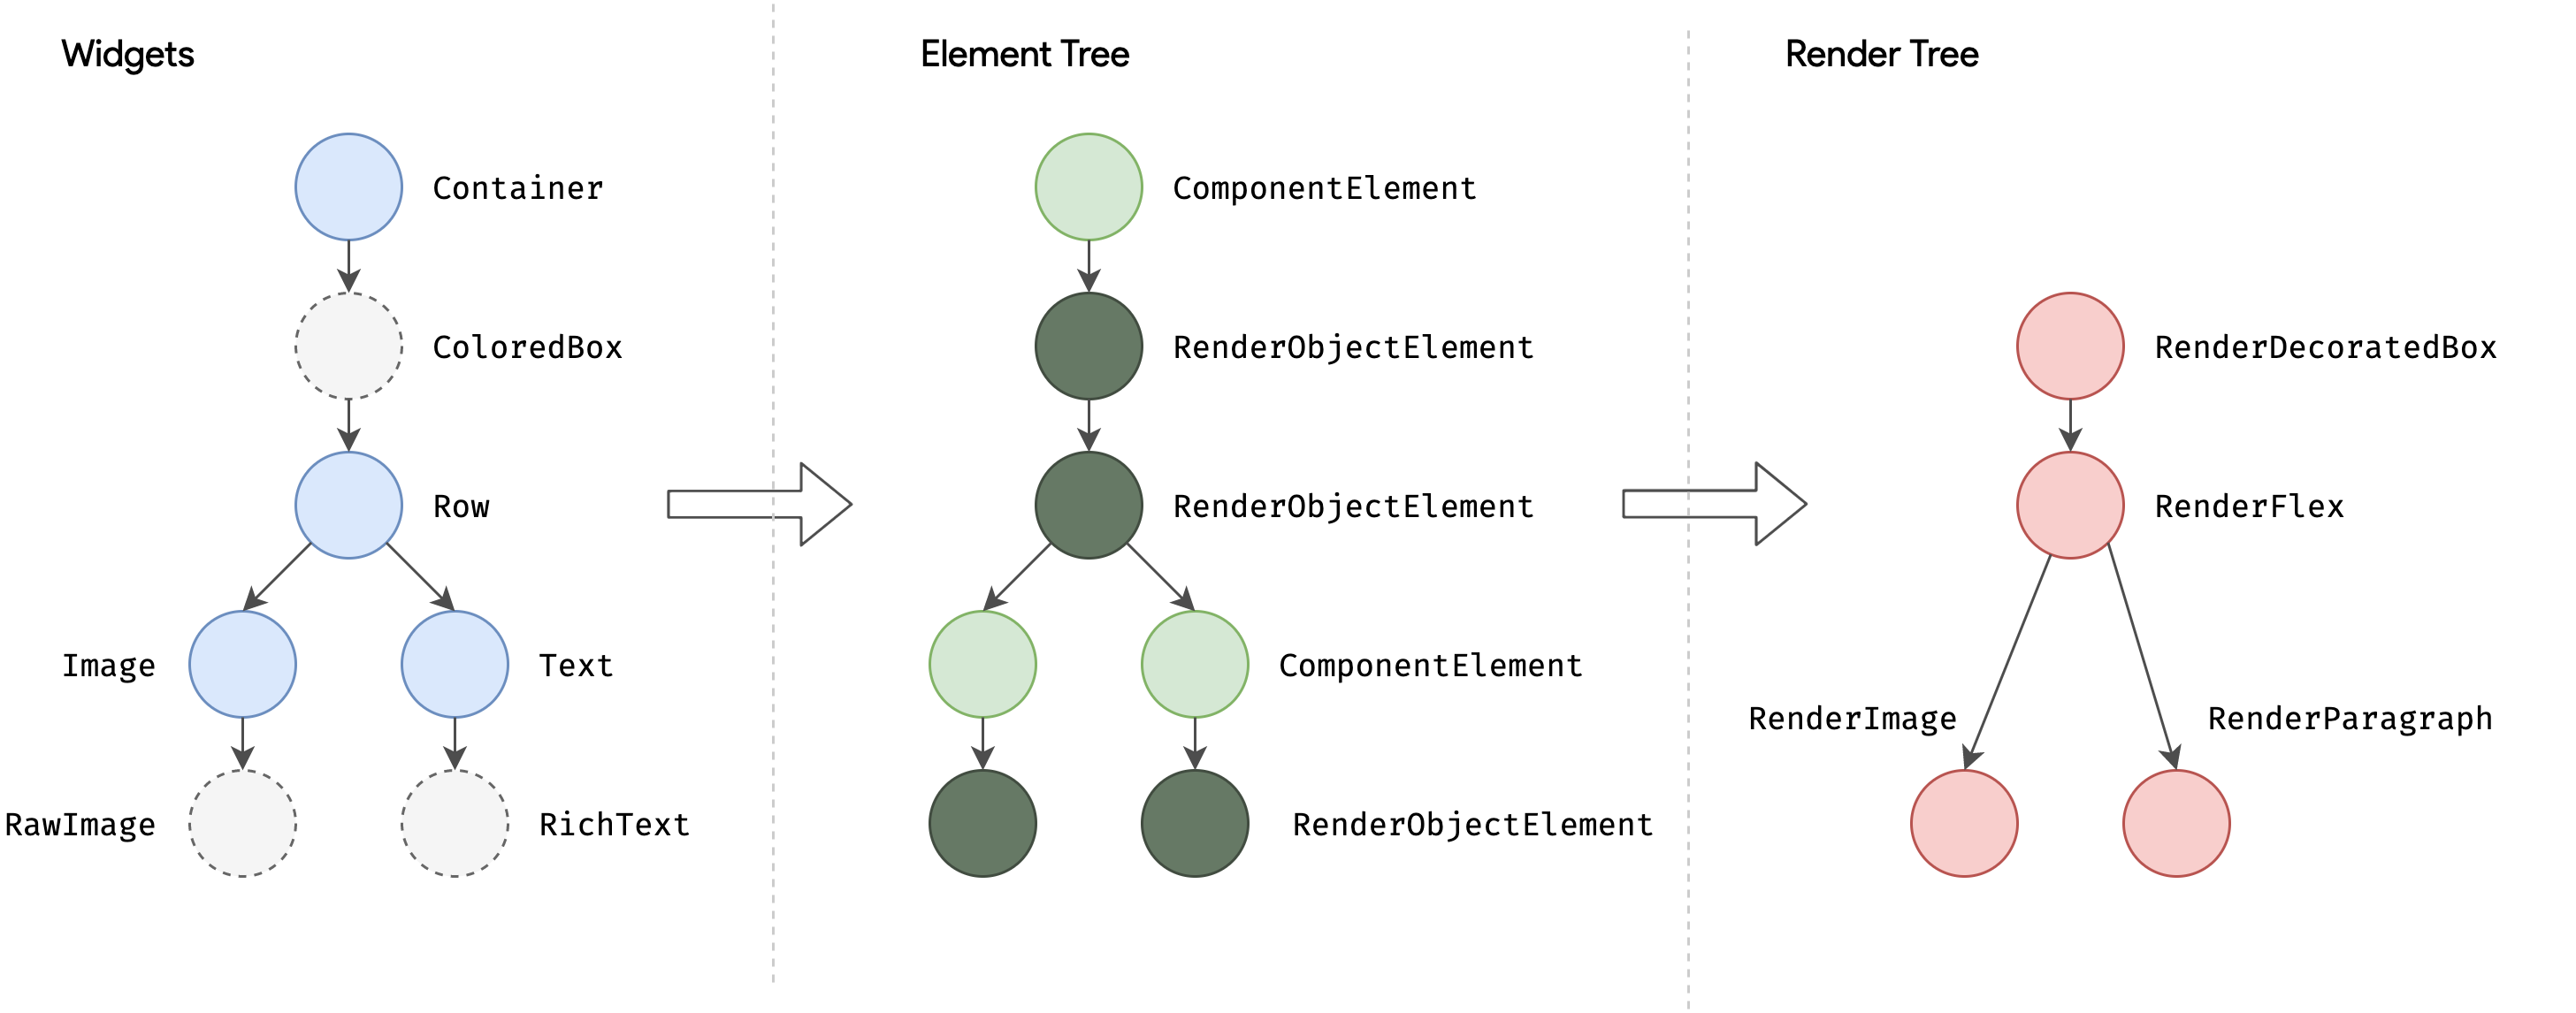
\includegraphics[width=\textwidth]{Flutter_trees}
    \caption[I tre alberi di Flutter]{Flutter usa tre alberi logici come rappresentazione delle proprie strutture: uno per i \textit{widget}, uno per gli \textit{element} e infine quello di \textit{render}.\footnotemark}
    \label{fig:flutter-trees}
\end{figure}
\footnotetext{Fonte: \url{https://docs.flutter.dev/resources/architectural-overview}}

L'albero di \textit{render} è una delle tre strutture logiche che Flutter usa per descrivere i propri oggetti e le proprie interfacce grafiche: il \textit{widget tree} rappresenta gli elementi di un \textit{widget} come uno \textit{stack} di \textit{widget}, messi in relazione con il loro elemento padre e i loro elementi figli. Nel caso del \textit{widget tree} rappresentato in figura \ref{fig:flutter-trees} esso rappresenta un \verb+Containter+ che contiene un \verb+ColoredBox+ che a sua volta contiene una \verb+Row+ e via dicendo. I \textit{widget} sono per definizione immutabili, quindi una modifica richiede necessariamente una distruzione e successiva ricreazione del \textit{widget} interessato.

\begin{lstlisting}[language=dart, caption={Codice rilevante per la parte grafica dell'\textit{app} di esempio di Flutter}]
    Widget build(BuildContext context) {
        return Scaffold(
          appBar: AppBar(
            title: Text(widget.title),
          ),
          body: Center(
            child: Column(
              mainAxisAlignment: MainAxisAlignment.center,
              children: <Widget>[
                const Text(
                  'You have pushed the button this many times:',
                ),
                Text(
                  '$_counter',
                  style: Theme.of(context).textTheme.headline4,
                ),
              ],
            ),
          ),
          floatingActionButton: FloatingActionButton(
            onPressed: _incrementCounter,
            tooltip: 'Increment',
            child: const Icon(Icons.add),
          ), // This trailing comma makes auto-formatting nicer for build methods.
        );
    }
\end{lstlisting}

Il codice precedente produce il seguente risultato (e il seguente \textit{widget tree}):

\begin{figure}[H]
    \centering
    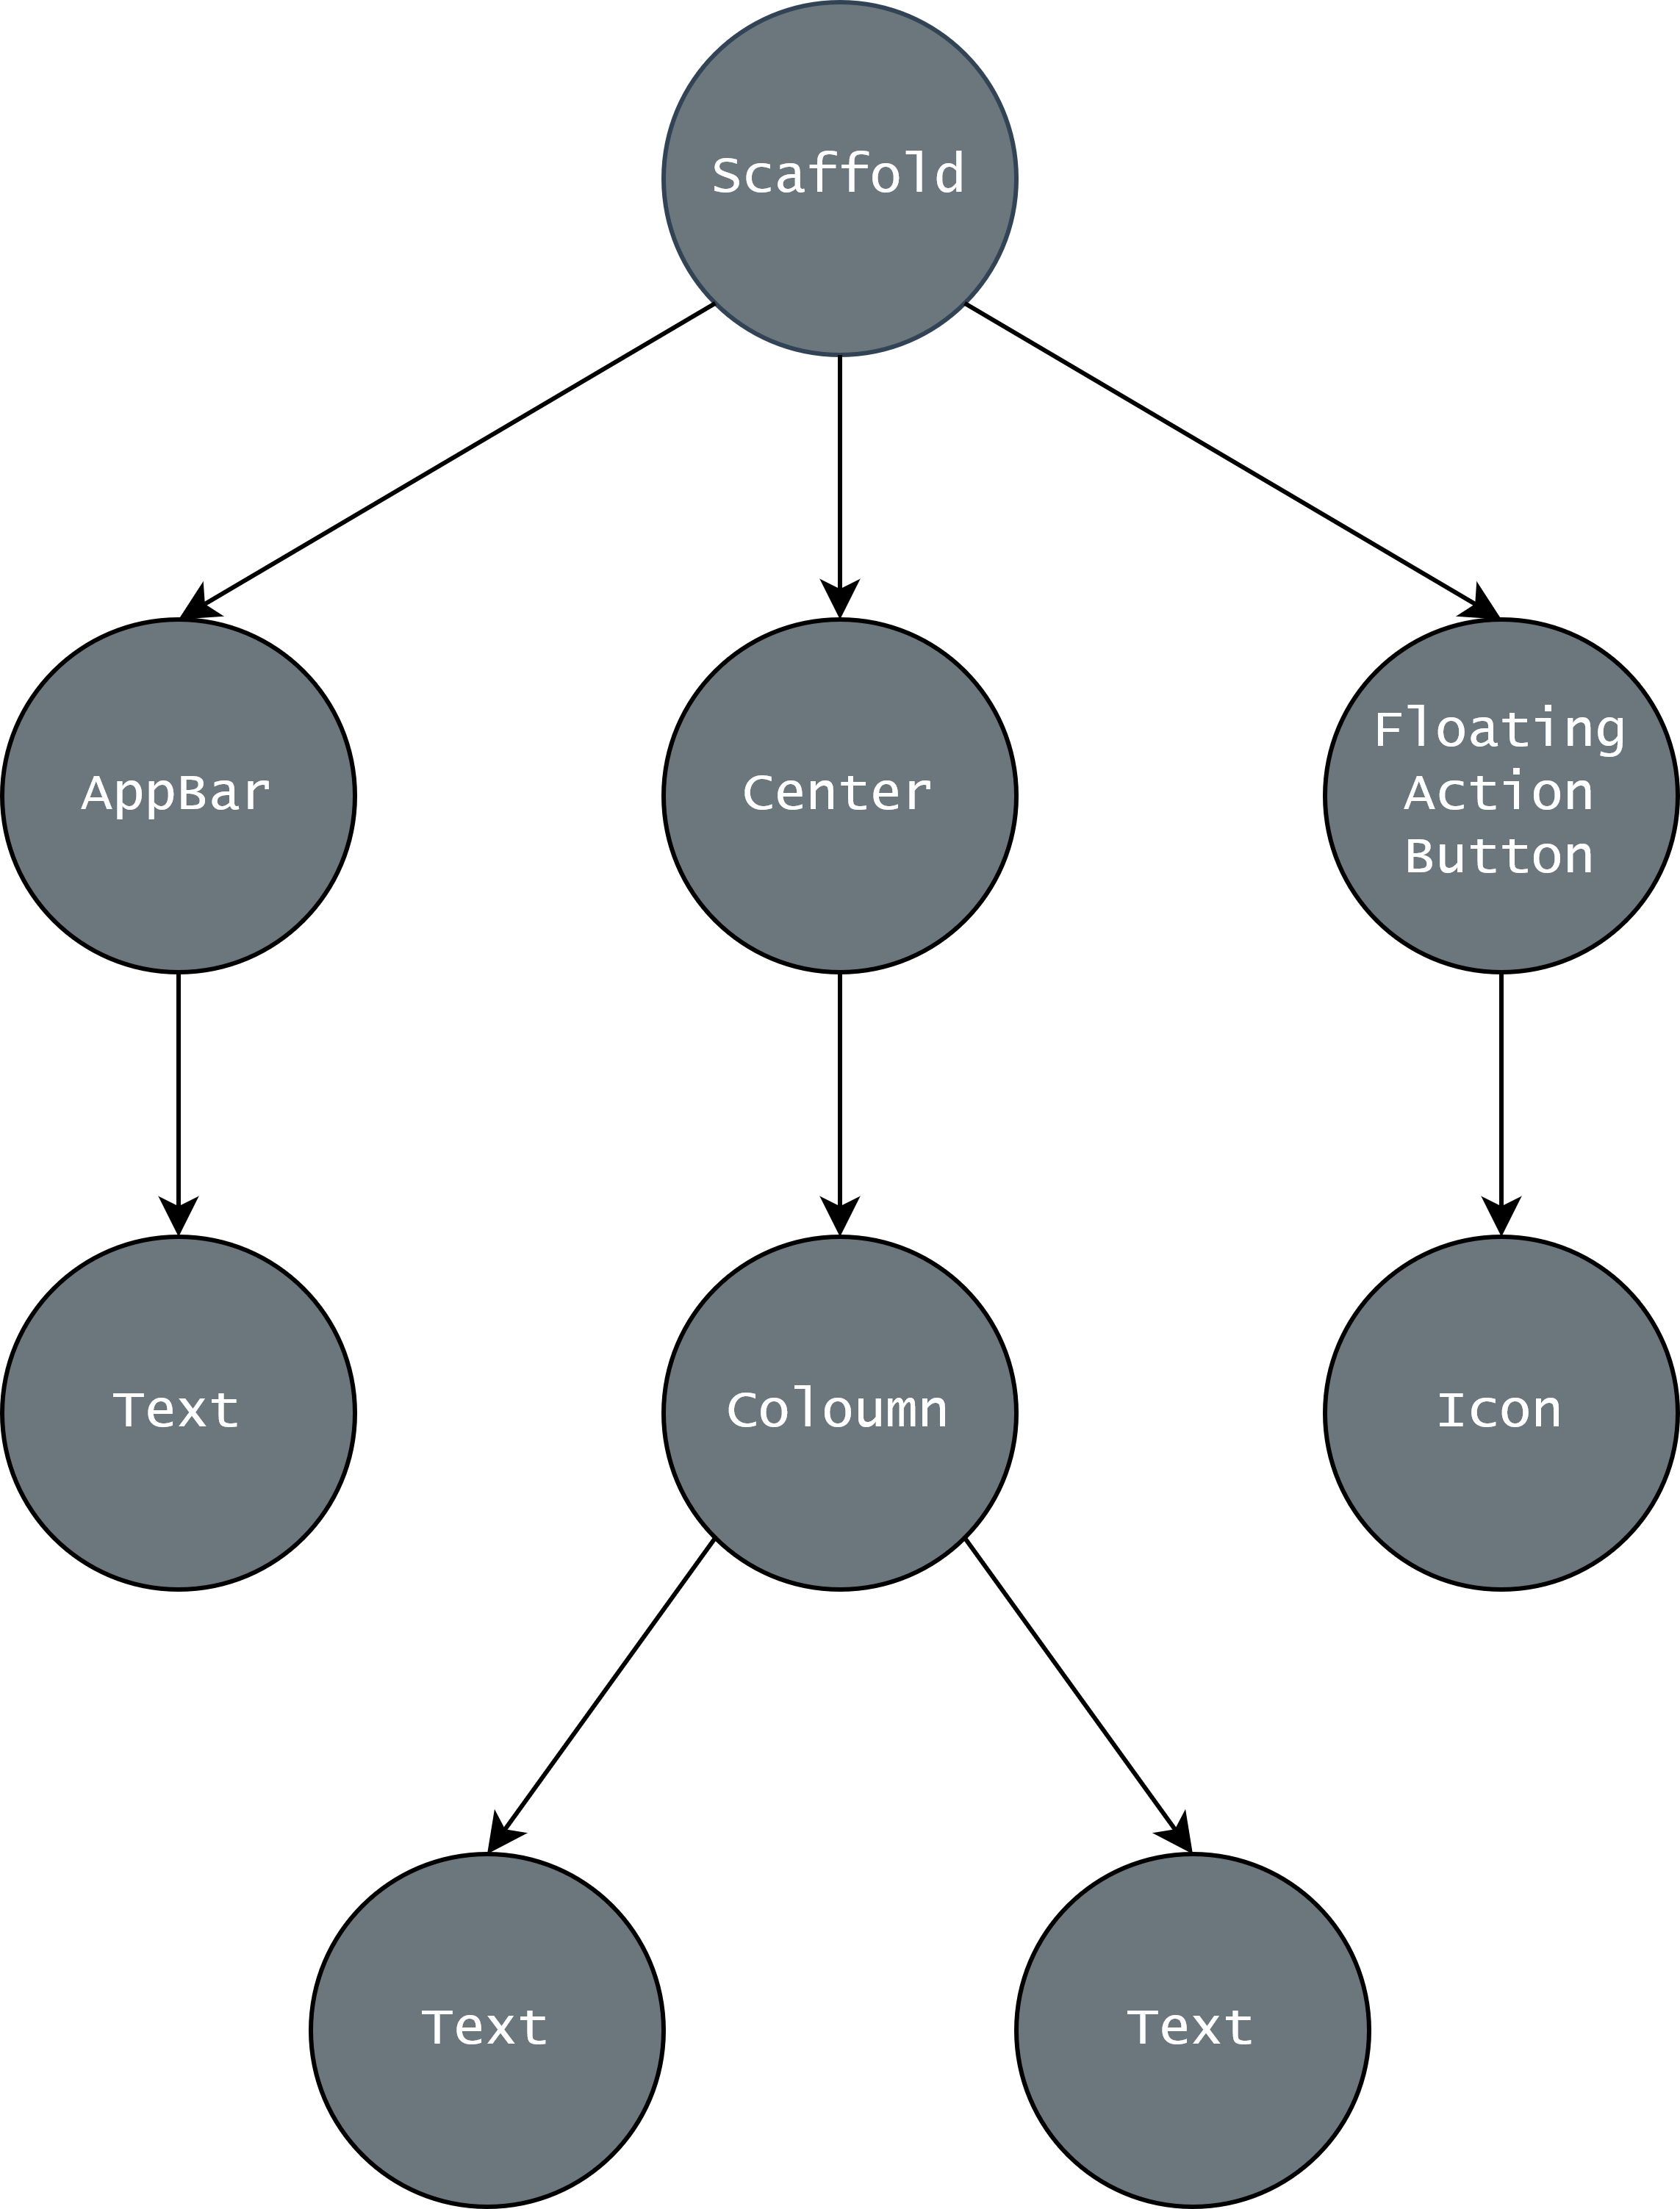
\includegraphics[height=8cm]{app_esempio_render_tree.png}\hspace{15mm}
    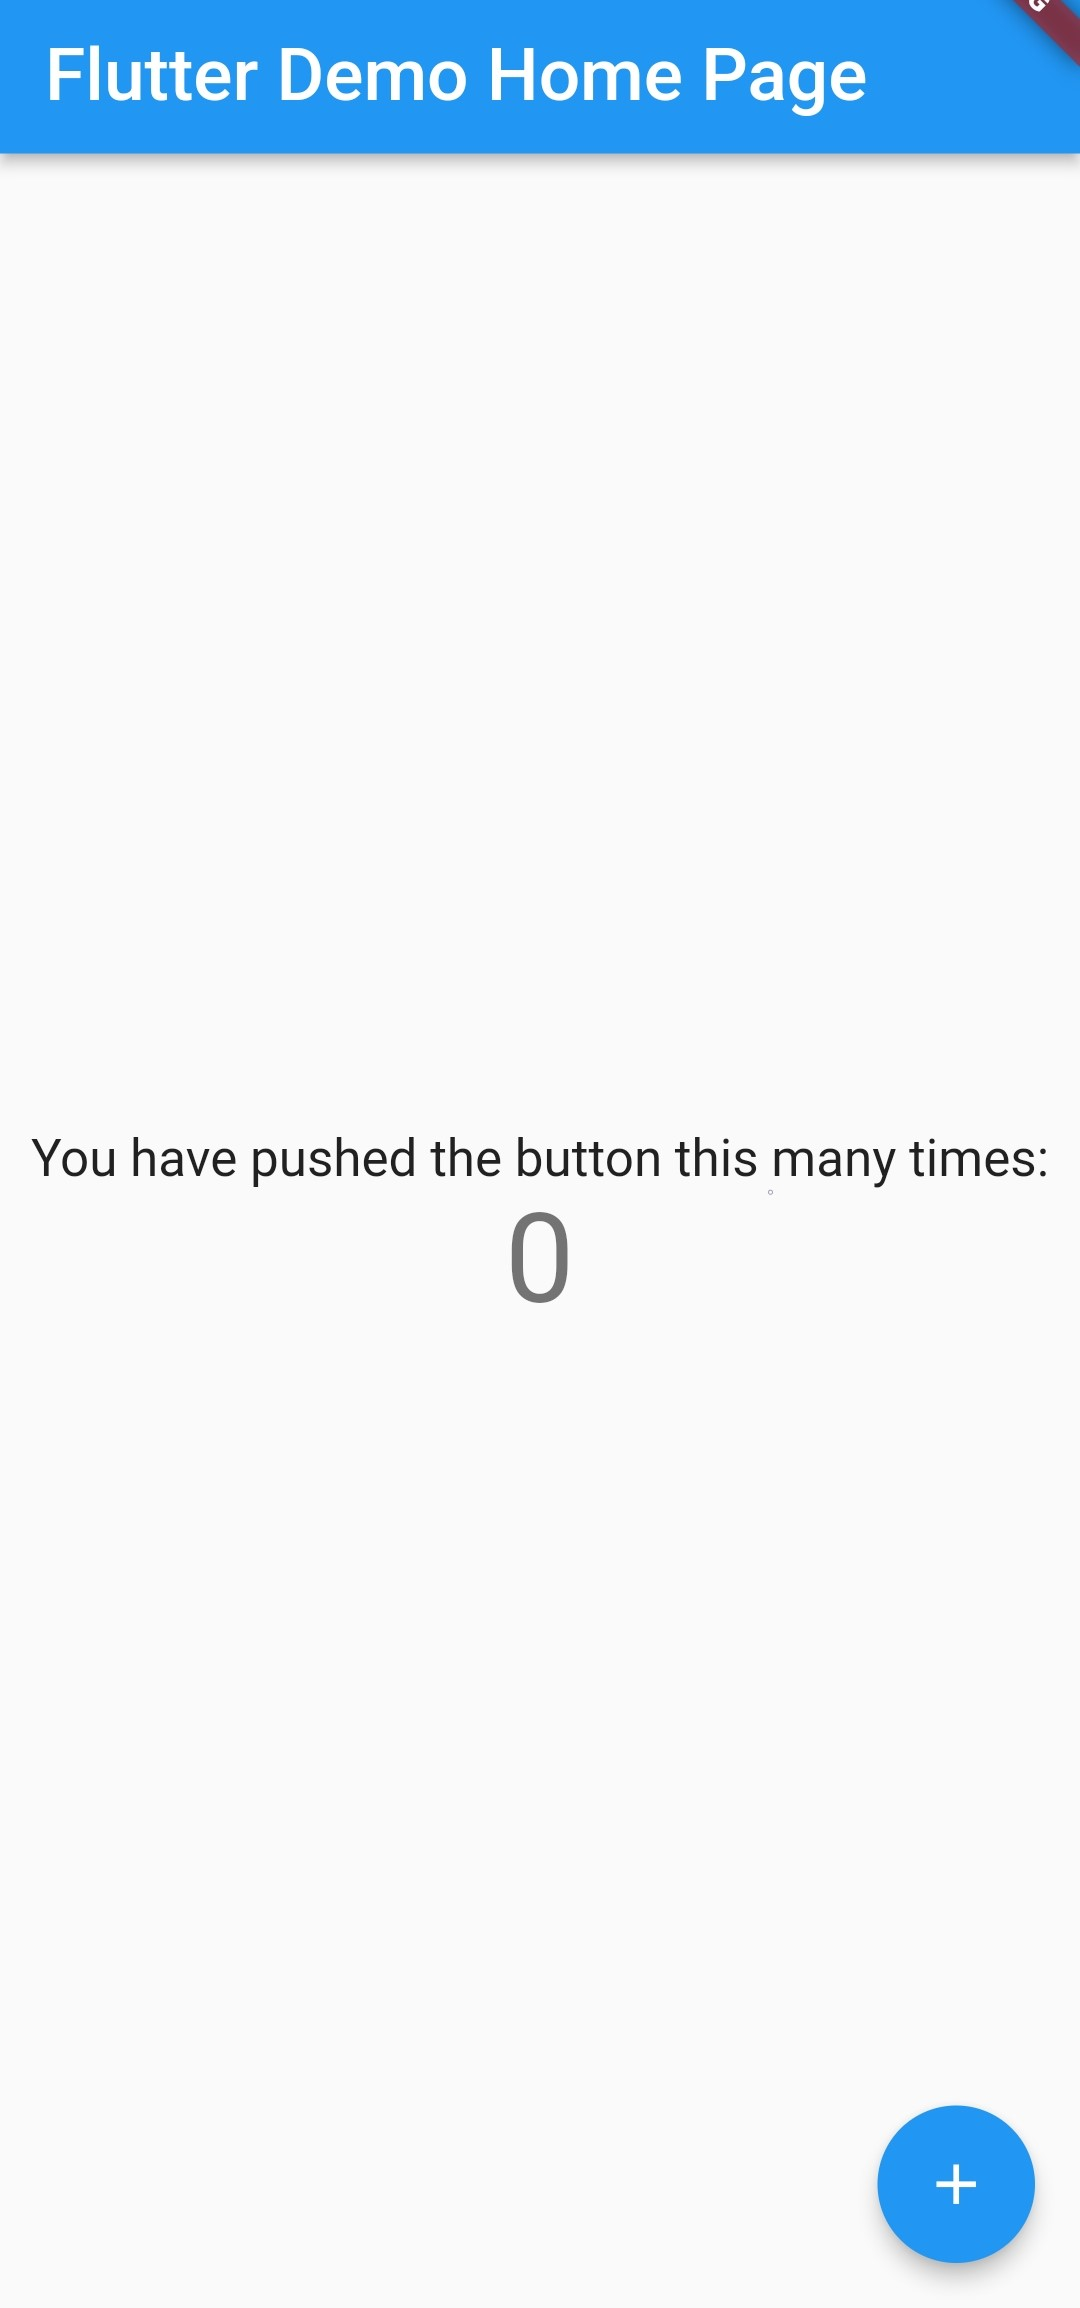
\includegraphics[height=8cm]{flutter_app_default.jpg}
    \caption[\textit{Widget tree} app esempio]{Il \textit{widget tree} dell'applicazione di esempio di Flutter e il suo risultato su Android}
\end{figure}

Per quanto riguarda le dimensioni delle varie componenti Flutter ragiona come segue: i padri passano ai figli (dall'altro verso il basso del \textit{widget tree}) dei \textit{"constraints"}, ovvero le dimensioni massime oltre le quali non possono cresce di dimensione, e i figli passano quindi ai padri (dal basso verso l'alto del \textit{widget tree}) le proprie dimensioni.\\
Il \textit{widget tree} è quello più importante da tenere a mente, e che più direttamente si interfaccia con il codice scritto dal programmatore. Torniamo però alla figura \ref{fig:flutter-trees} per parlare brevemente degli altri due alberi: l'\textit{element tree} rappresenta gli elementi che, a differenza dei \textit{widget}, sono mutabili e vengono definiti come "un'istanza di un \textit{Widget} in una particolare posizione dell'albero". Gli elementi sono responsabili di aggiornare l'interfaccia utente e fungono da ponte tra \verb+Widget+ e \verb+Render Object+.\\
Il \textit{render tree} rappresenta i \verb+Render Object+ e viene interpellato dal \textit{framework} per disegnare i componenti dell'interfaccia grafica. Una singola istanza di \verb+Render Object+ contiene tutte le informazioni riguardanti dimensioni, colori e logiche di \textit{layout} di un \verb+Widget+.\\
Abbiamo accennato che i \textit{widget} quando chiamano stato richiamano il proprio metodo \verb+build+ che provoca quindi una ricostruzione del \textit{widget} stesso. Questi \textit{widget} si chiamano \textit{"stateful}, e sono in diretta contrapposizone con quelli incapaci di modificarsi durante l'esecuzione, chiamati \textit{"stateless"}. 

\begin{lstlisting}[language=dart, label={lst:stateful_widget}, caption={Creazione \textit{stateless widget}}]
class MyApp extends StatelessWidget {
  //stateless widget che fa da radice per l'applicazione
  const MyApp({super.key});

  @override
  Widget build(BuildContext context) {
    return MaterialApp(
        home: const MyHomePage(title: 'Flutter Demo Home Page'),
    );
  }
}

class MyHomePage extends StatefulWidget {
  //qui passiamo allo stateful widget
  const MyHomePage({super.key, required this.title});
  final String title;

  @override
  //e qui creiamo lo stato vero e proprio
  State<MyHomePage> createState() => _MyHomePageState();
}


class _MyHomePageState extends State<MyHomePage> {
  int _counter = 0;

  void _incrementCounter() {
    //quando viene chiamata questa funzione viene
    //richiamato il metodo build, di fatto cambiando lo stato 
    //del widget e provocando un render dell'applicazione
    setState(() {
      _counter++;
    });
  }

  @override
  Widget build(BuildContext context) {}
}
\end{lstlisting}

Si nota immediatamente che l'uso degli \textit{stateful widget} provoca la scrittura di codice ridondante e si è quindi deciso di arginare questo problema, aumentando al contempo la condivisione di codice tra i \textit{widget}, introducendo i Flutter Hooks (ispirati dagli \textit{hooks} di React).
Vediamo quindi la riscrittura del codice mostrato in estratto \ref{lst:stateful_widget} opportunamente modificato usando un \verb+HookWidget+:

\begin{lstlisting}[language=dart, caption={Creazione \textit{hook widget}}]
class MyApp extends StatelessWidget {
  //stateless widget che fa da radice per l'applicazione
  const MyApp({super.key});

  @override
  Widget build(BuildContext context) {
    return MaterialApp(
        home: const MyHomePage(title: 'Flutter Demo Home Page'),
    );
  }
}

class MyHomePage extends HookWidget {
  //basta questa classe per fare tutti gli step
  //necessari al cambio di stato

  const MyHomePage({super.key, required this.title});
  final String title;

  Widget  build (BuildContext context){
    //_counter viene inizializzato a zero e reso
    //l'hook per il cambio di stato, quindi quando
    //il suo valore cambia viene provocato un rebuild
    final _counter = useState(0)

    return Scaffold(
      appBar: AppBar(),
      body: Center(),
      floatingActionButton: FloatingActionButton(
        //qui il valore di _counter cambia
        //provocando una rebuild
        onPressed: () => _counter.value++,
      )
    )
  }
}
\end{lstlisting}

\subsubsection{Method Channels}
I \textit{method channel} nascono per uno scopo: utilizzare codice nativo tramite Flutter, ad esempio chiamare \api{} \textit{platform-specific} come Kotlin o Java per Android, Swift per iOS o C++ su Windows.\\
Flutter non usa queste funzionalità tramite generazione di codice e preferisce un approccio basato sullo scambio di messaggi. Vediamo quindi un esempio di utilizzo per ottenere, tramite Java, il valore di carica della batteria di un dispositivo Android.\\
Per prima cosa è necessario agire sull'Android \textit{manifest} inserendo il nome dell'applicazione di Flutter (in questo caso \verb+batterylevel+). L'applicazione si può creare con il comando \verb+flutter create nome_applicazione+.

\begin{lstlisting}[language=XML, firstnumber=1,caption={Android \textit{manifest}}]
<manifest xmlns:android="http://schemas.android.com/apk/res/android"
  package="com.example.batterylevel">
\end{lstlisting}

A questo punto si vanno a costruire gli "agganci" per il \textit{method channel} in codice nativo, in questo caso quindi nell'attività principale di Java:

\begin{lstlisting}[language=Java, firstnumber=1,caption={Java \textit{main activity}}]
  public class MainActivity extends FlutterActivity {
    //"samples.flutter.dev/battery" e' il nome del method channel
    //come definito in main.dart
    private static final String CHANNEL = "samples.flutter.dev/battery";

    @Override
    public void configureFlutterEngine(@NonNull FlutterEngine flutterEngine) {
        super.configureFlutterEngine(flutterEngine);
        new MethodChannel(flutterEngine.getDartExecutor().getBinaryMessenger(), CHANNEL)
                .setMethodCallHandler(
                        (call, result) -> {
                            //Questo e' il metodo invocato nel main
                            //sfruttiamo la stringa 'getBatteryLevel' per invocarlo
                            if (call.method.equals("getBatteryLevel")) {
                                //il metodo vero e proprio in Java
                                int batteryLevel = getBatteryLevel();

                                if (batteryLevel != -1) {
                                    result.success(batteryLevel);
                                } else {
                                    result.error("UNAVAILABLE", "Battery level not available.", null);
                                }
                            } else {
                                result.notImplemented();
                            }
                        }

                );
    }

    private int getBatteryLevel() {
      //metodo che ritorna il valore di batteria del dispositivo
    }

\end{lstlisting}

Infine ci occupiamo di lanciare il messaggio da Flutter invocando il metodo:

\begin{lstlisting}[language=dart, firstnumber=1,caption={Dart \textit{main}}]
  class MyHomePage extends HookWidget {
  const MyHomePage({super.key});
  //creo e definisco il method channel
  static const platform = MethodChannel('samples.flutter.dev/battery');

  @override
  Widget build(BuildContext context) {
    var batteryLevel = useState('Unknown battery level.');

    return Material(
      child: Center(
        child: Column(
          mainAxisAlignment: MainAxisAlignment.spaceEvenly,
          children: [
            ElevatedButton(
              onPressed: () async {
                try {
                  //qui avviene l'effettiva invocazione del method channel
                  //che provoca una chiamata in Java
                  final int result =
                      await platform.invokeMethod('getBatteryLevel');
                  batteryLevel.value = 'Battery level at $result % .';
                } on PlatformException catch (e) {
                  batteryLevel.value =
                      "Failed to get battery level: '${e.message}'.";
                }
              },
              child: const Text('Get Battery Level'),
            ),
            Text(batteryLevel.value),
          ],
        ),
      ),
    );
  }
}
\end{lstlisting}


\subsection{Realtà aumentata}
Uno dei punti centrali di questa tesi è la realtà aumentata e gli ancoraggi che è possibile posizionare all'interno di uno spazio tridimensionale, ed è quindi intelligente presentare preventivamente l'argomento e i concetti chiave.\\
La realtà aumentata consiste nel prendere lo spazio tridimensionale reale e trasporlo, tramite tecniche di mappatura, in formato digitale per poi poterci effettuare delle manipolazioni tramite \textit{software}. Ad esempio è possibile, nell'applicazione di Ikea, inquadrare il proprio salotto e posizionarci dei modelli poligonali\footnote{Detti anche \textit{asset} poligonali, prendono questo nome perché nel mondo della modellazione digitale tridimensionale le entità sono composte da triangoli adiacenti tra loro (poligoni appunto) che costruiscono una figura volumetrica. Questo perché il triangolo è la più semplice forma bidimensionale esistente, e quindi la meno esosa da calcolare.} della mobilia venduta dal colosso svedese.\\

\todo{} inserire pic ikea\\

Sebbene sia possibile immaginare lo spazio virtuale come un cubo vuoto all'interno del quale posizionare \textit{asset}, vengono applicate delle semplificazioni logiche per una questione di complessità ed efficienza di calcolo: lo spazio viene processato come una serie di piani bidimensionali sovrapposti a diverse altezze (una sorta di \textit{stack} di battaglie navali) e gli ancoraggi si legano quindi a una coppia di coordinate \textit{(x,y)} relativa al piano più la coordinata \textit{(z)} del piano stesso. Esistono inoltre piani orizzontali e verticali (non a caso alcune delle funzioni chiave di ARCore e ARKit servono a identificare gli spazi lisci).

\begin{figure}[H]
  \centering
  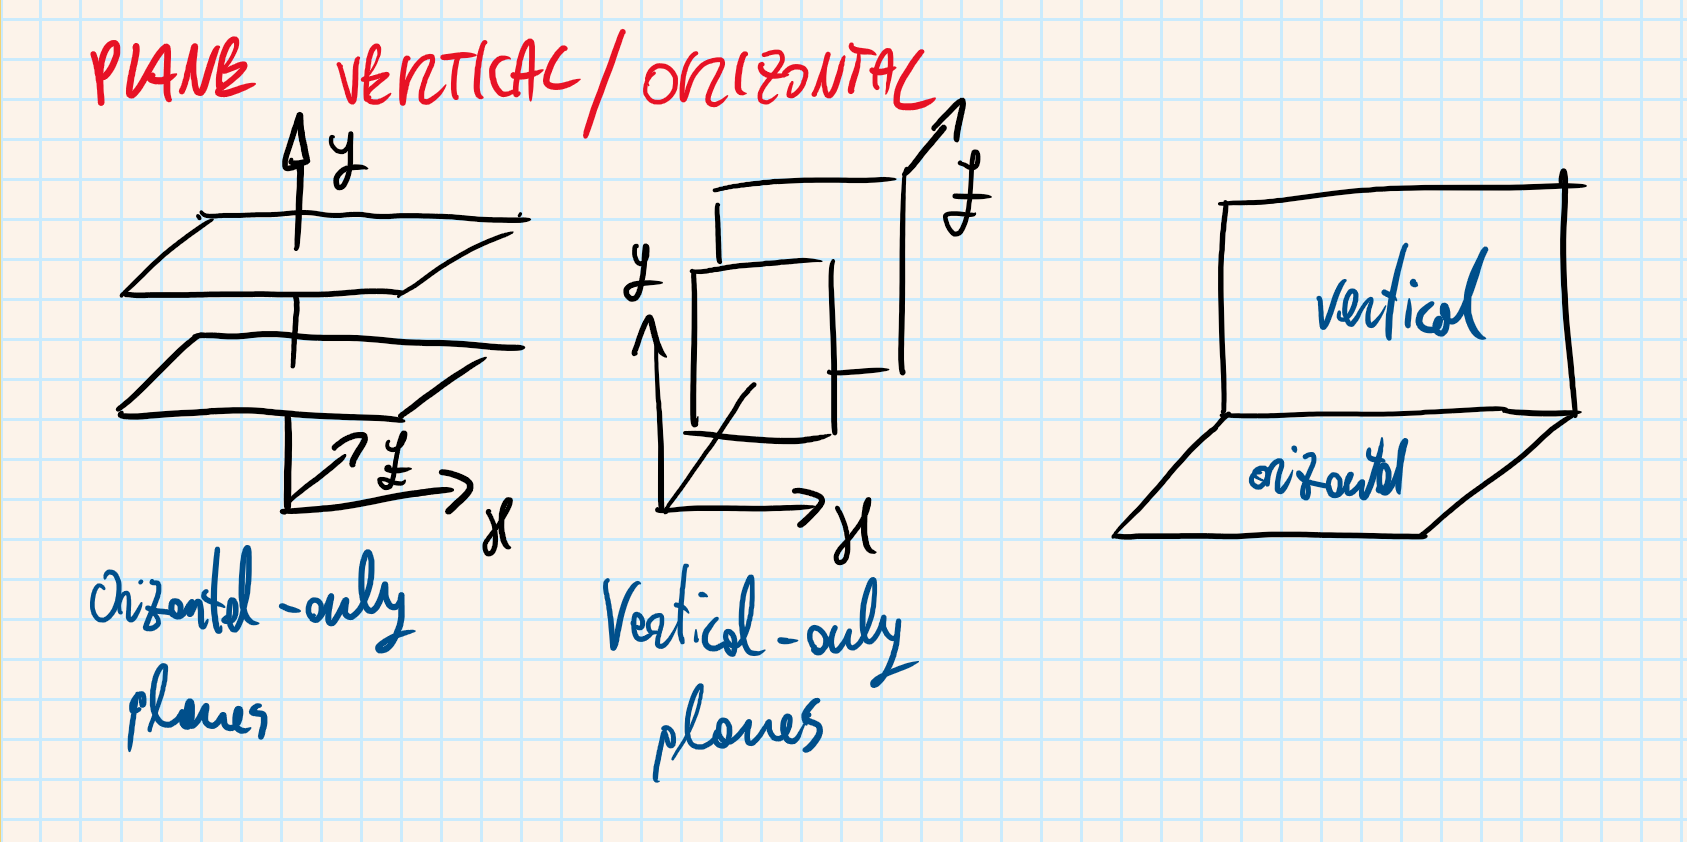
\includegraphics[width=\textwidth]{planes3D_temp}
  \caption[Piani in realtà aumentata]{caption \todo}
\end{figure}

Nella maggior parte dei casi è bene legare a un ancoraggio multiple entità diverse, questo perchè la \textit{pose} degli oggetti (ovvero rotazione verticale e orizzontale) è legata a quella della \textit{anchor} associata. Di conseguenza se vogliamo rappresentare in una stanza un insieme realistico di mobili (o meglio, di modelli poligonali e quindi gemelli digitali di mobili), se li leghiamo a un ancoraggio centrale rispetto alla stanza tutti gli elementi avranno sempre una posizione relativa corretta tra di loro. Se invece ogni elemento ha la sua \textit{anchor} potremmo vedere rotazioni errate oppure potrebbero spostarsi anche di qualche metro rispetto alla loro posizione originale.

\begin{figure}[H]
  \centering
  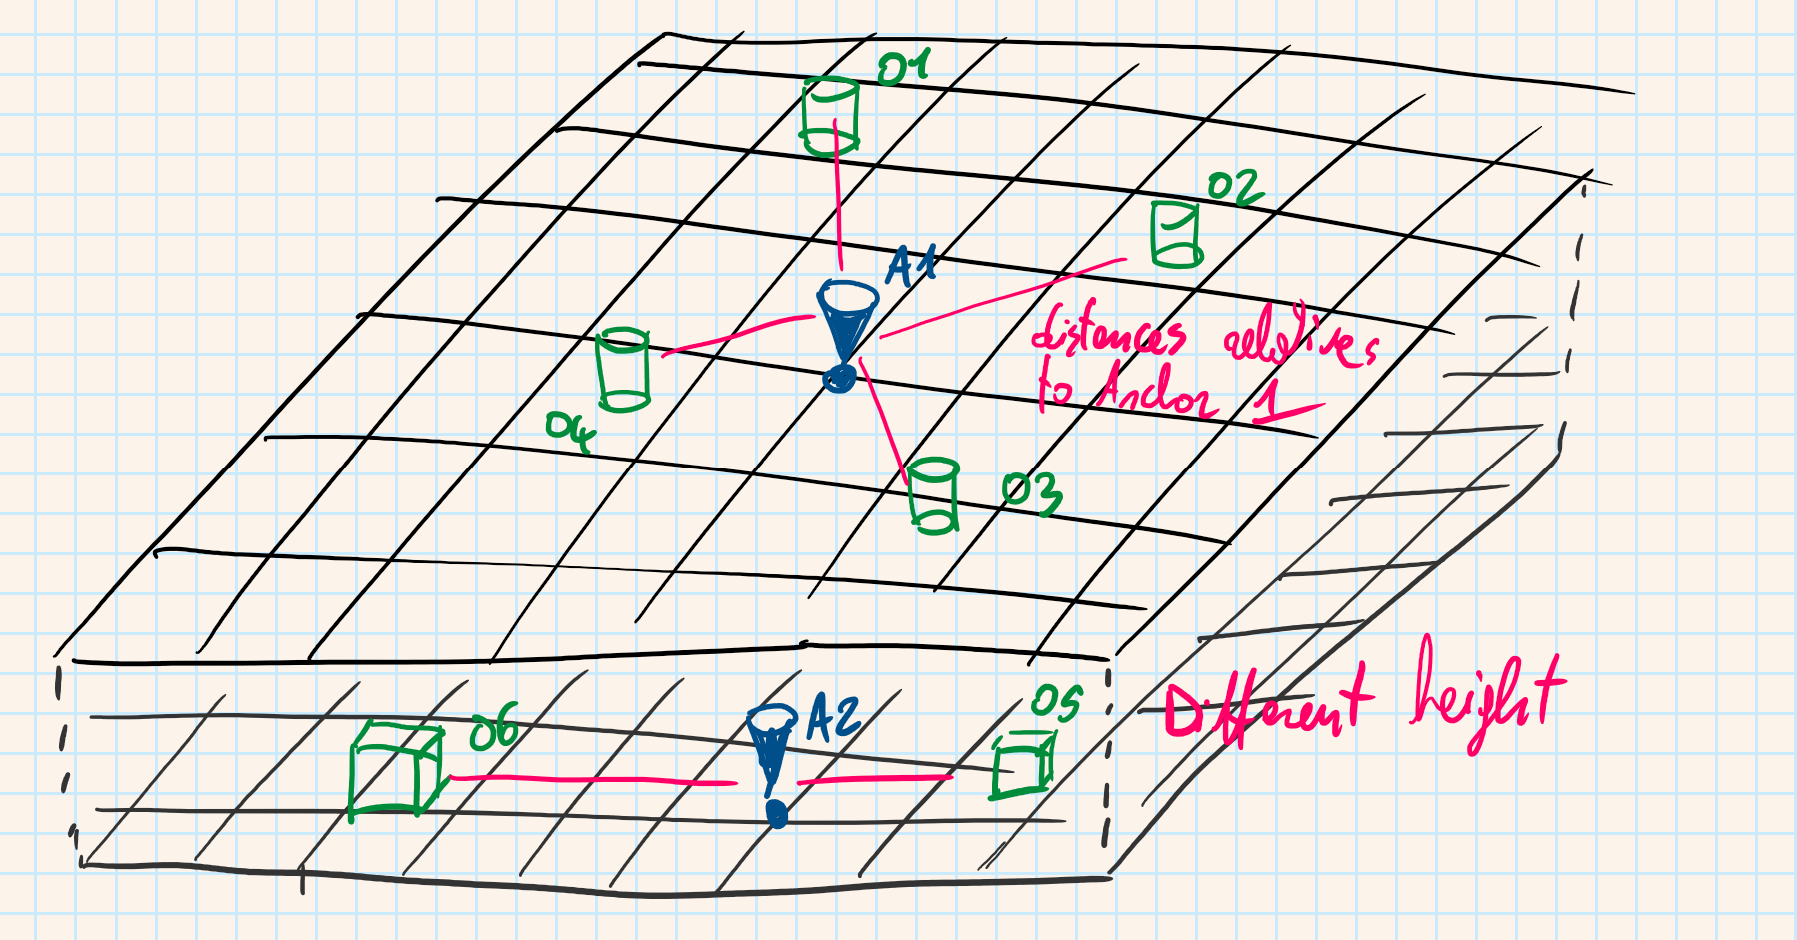
\includegraphics[width=\textwidth]{anchors_temp}
  \caption[Ancoraggi singoli per multipli elementi]{caption \todo}
\end{figure}

\subsection{Azure ToolKit}
Azure è l'ombrello sotto al quale vivono tutti i servizi \textit{cloud} di Microsoft esterni al pacchetto Office 365, e comprendono \textit{database} relazionali con scalabilità automatica (Azure SQL o Azure Cosmos DB), macchine virtuali remote (Virtual Machines e Azure Virtual Desktop) fino a funzionalità estremamente avanzate come Azure Kubernetes Service che fornisce un sistema automatizzato per rilasciare, scalare e gestire grandi applicativi \textit{sofware} (ad esempio per i \textit{data center}), oppure Azure Quantum che mette a disposizioni soluzioni per scrivere e far girare \textit{software} su \textit{hardware} quantistico.\\
Come si può notare la \textit{suite} Azure è indirizzata a utenti altamente specializzati e ancora più spesso a organizzazioni vere e proprie.

\begin{figure}[H]
  \centering
  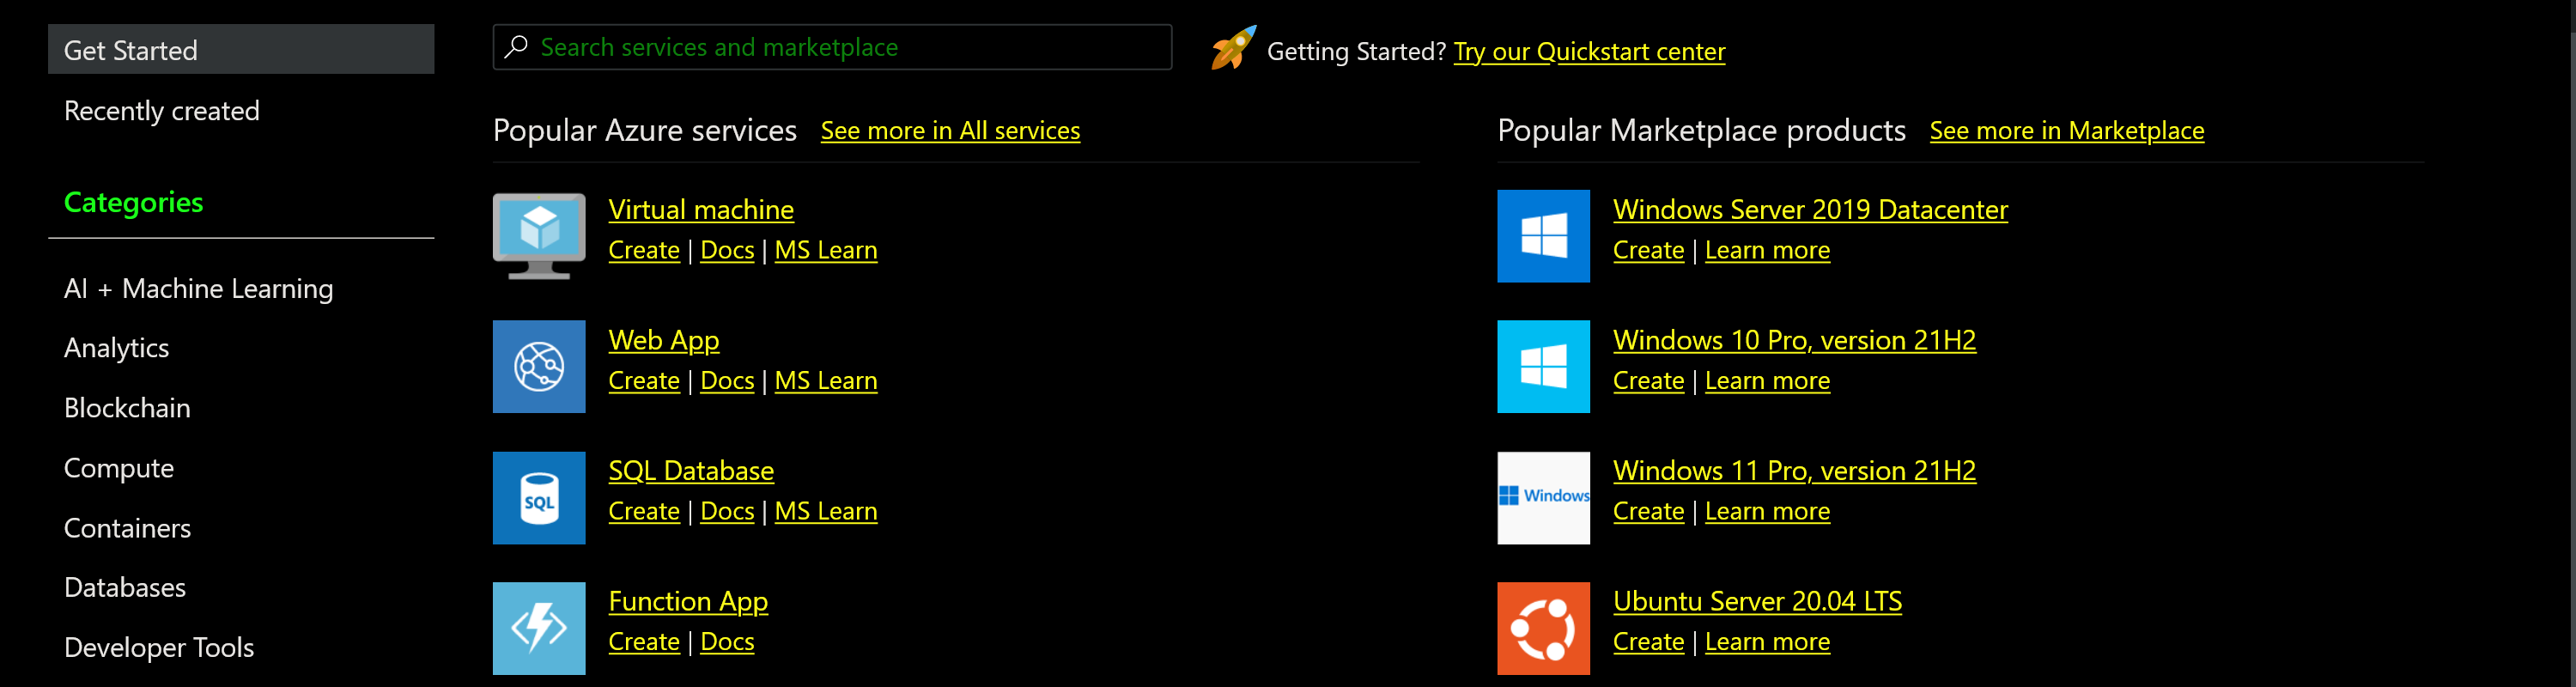
\includegraphics[width=\textwidth]{azure_resources}
  \caption[Azure Portal creazione risorse]{caption \todo}
\end{figure}

Per gli scopi di questo progetto ci serviremo di due degli strumenti forniti: l'Azure Portal e le \asa{}.\\
Il primo è semplicemente un portale online che serve a gestire, creare e monitorare tutte le risorse Azure legate a un \textit{account}, mentre le seconde sono il servizio di Microsoft per gestire ancoraggi geospaziali persistenti che possono anche essere utilizzati in un contesto di realtà aumentata.

\begin{figure}[H]
  \centering
  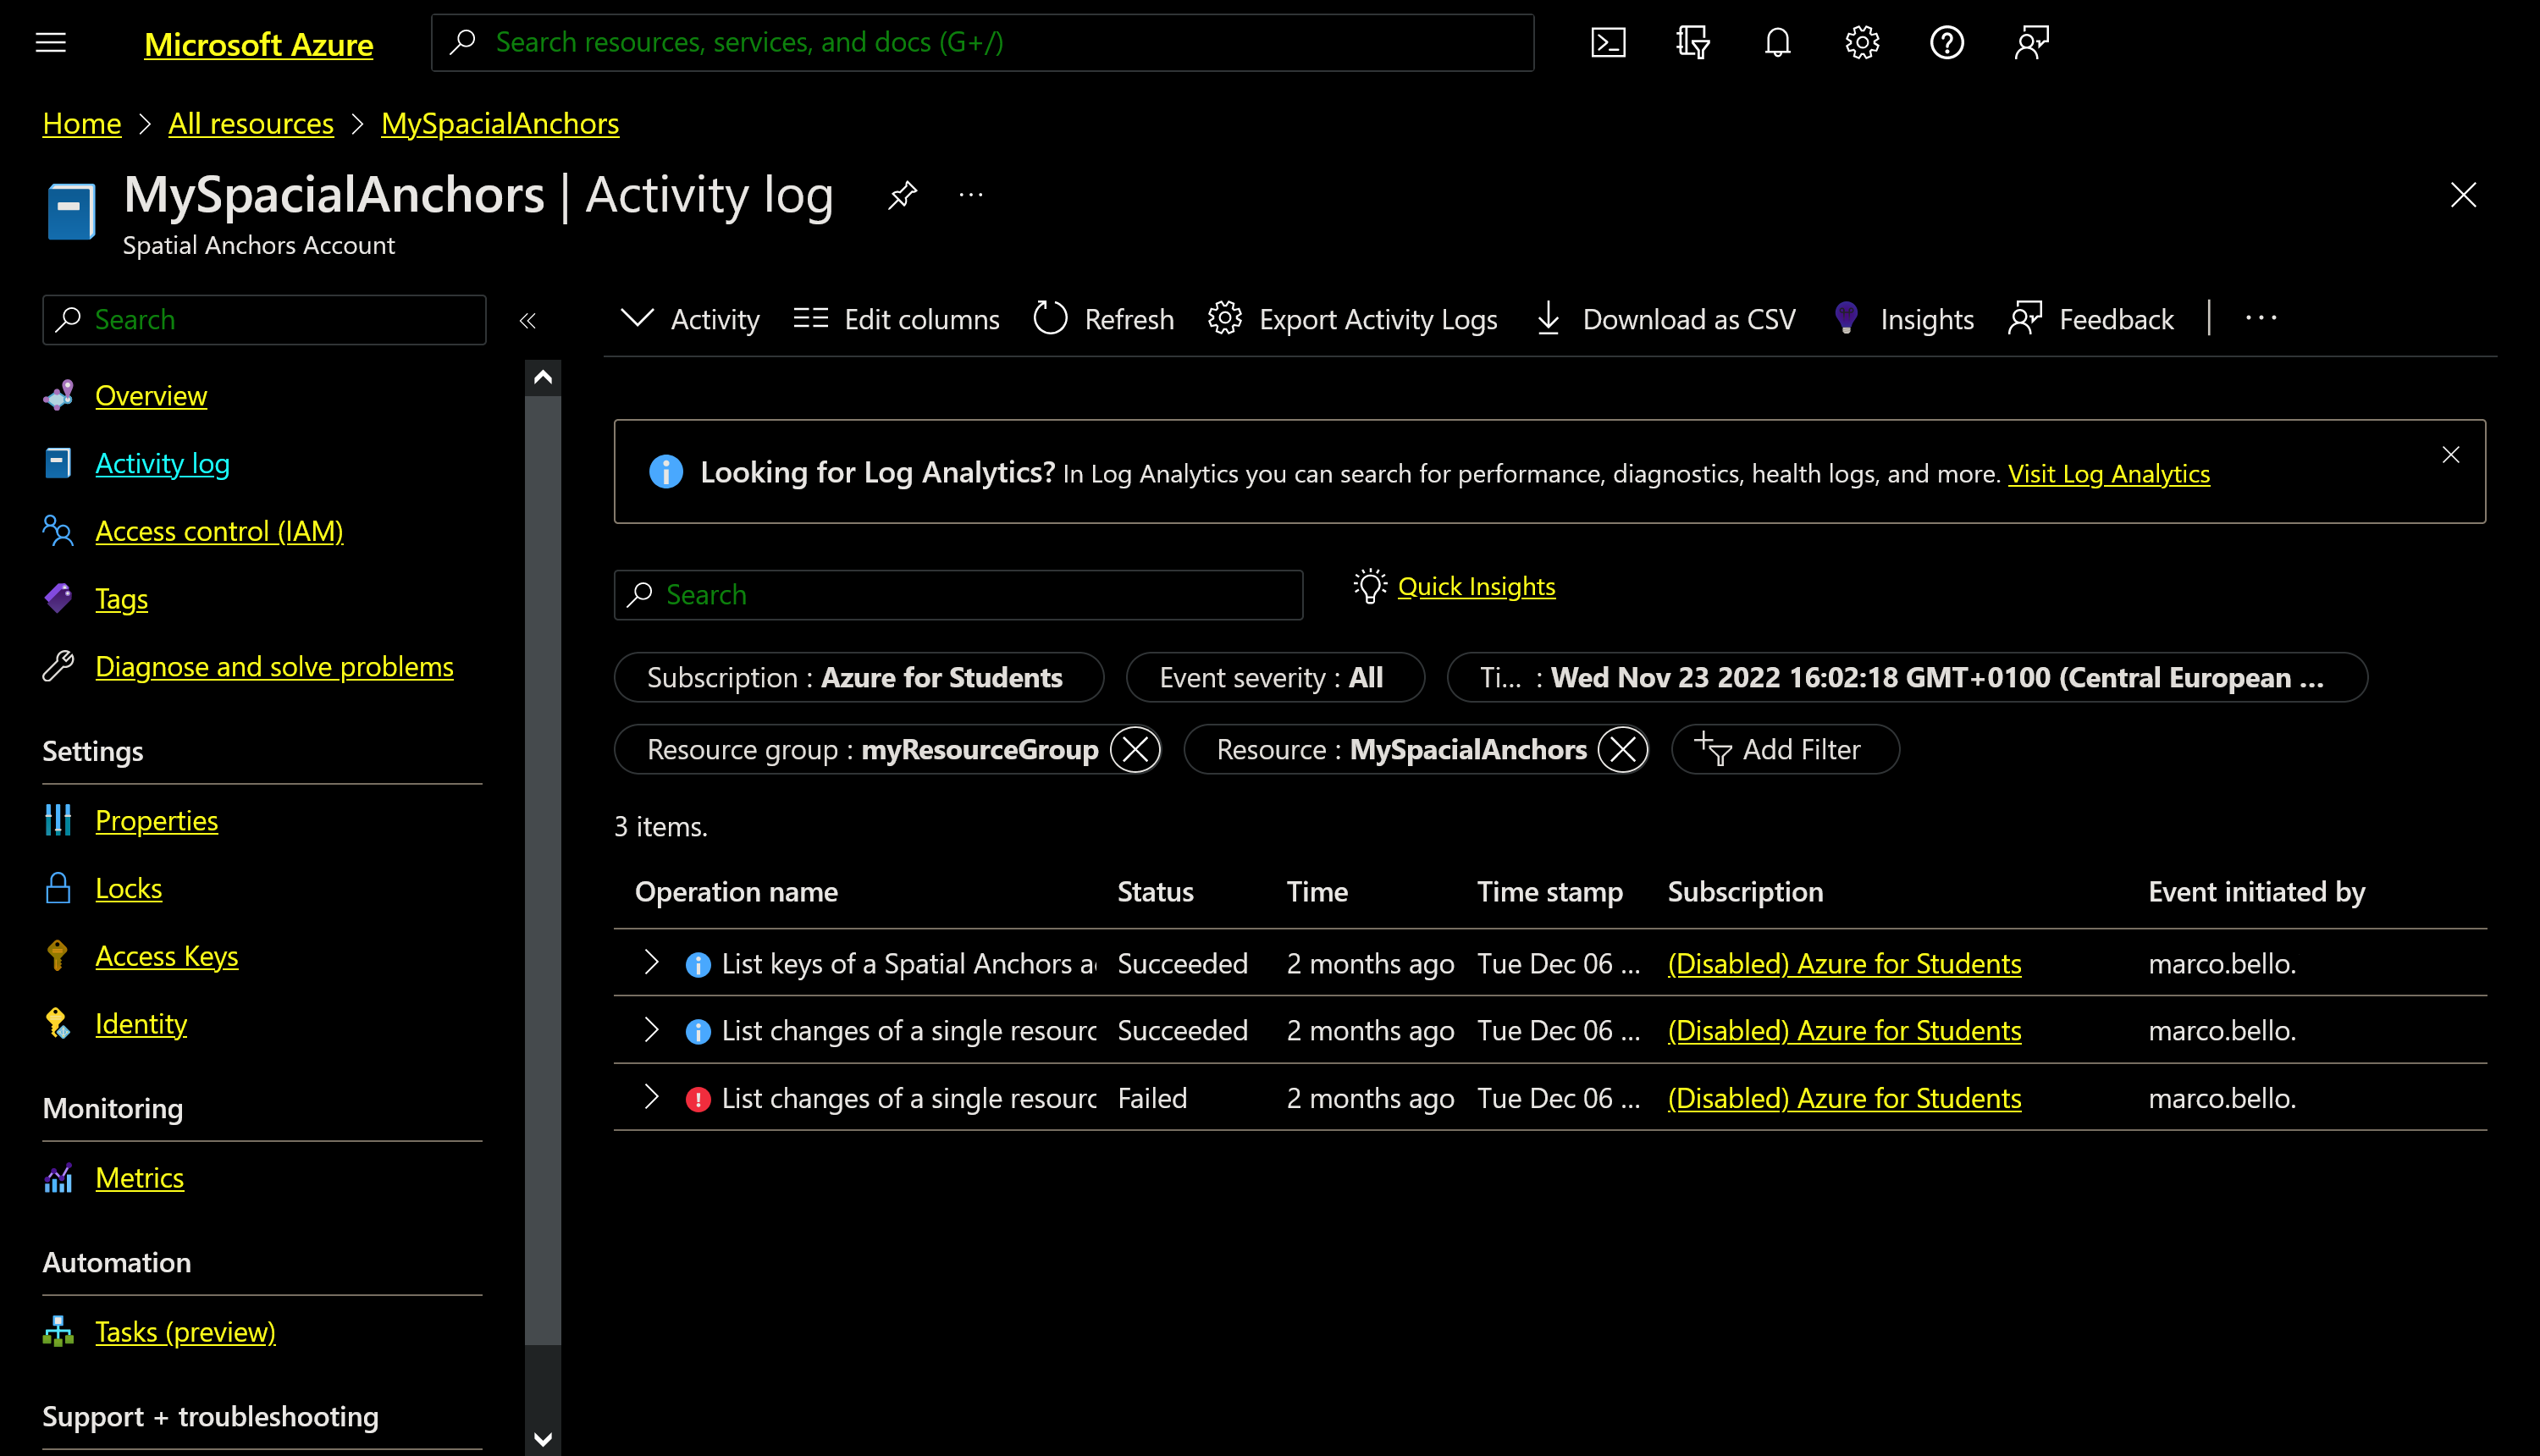
\includegraphics[width=\textwidth]{asa_azure_portal}
  \caption[Azure Portal]{caption \todo}
\end{figure}

Le \asa{} forniscono tre \sdk{}s, uno per Microsoft HoloLens, uno per iOS appoggiandosi su ARKit e uno per Android basato su ARCore, possono collegarsi tra loro creando relazioni che formano dei veri e propri percorsi (funzionalità usata spesso nel contesto degli \textit{asset} aziendali, ad esempio in una stessa linea produttiva) e possono essere contenuti dentro un \textit{resource group} di Azure che funge da contenitore di risorse dentro al quale esse vengono create e gestite.

\subsection{Framework realtà aumentata per Flutter}
Essendo lo scopo di questo stage, e quindi il caso di studio di questa tesi, l'implementazione di una vista in realtà aumentata (nello specifico sfruttando \asa{}) in un'applicazione preesistente sviluppata in Flutter, una grossa parte del lavoro svolto si è incentrato sullo studio dei \textit{framework} e/o \textit{plug-in} disponibili.\\
Sfortunatamente, complici la giovinezza di Flutter e la scarsa diffusione di tecnologie per la realtà aumentata, le opzioni disponibili sono alquanto ridotte:
\begin{itemize}
    \item \aplug{}: \textit{plugin}\footnote{Fonte: \url{https://pub.dev/packages/ar_flutter_plugin}} che punta a implementare le componenti in realtà aumentata in modalità \textit{cross-platform}, quindi adattandosi autonomamente ad Android e iOS (sfruttando tuttavia le Cloud Anchor di Google). Nasce partendo da due plugin più specializzati: 
    \begin{itemize}
        \item arcore\_flutter\_plugin per Android\footnote{Fonte: \url{https://github.com/giandifra/arcore_flutter_plugin}};
        \item arkit\_flutter\_plugin per iOS\footnote{Fonte: \url{https://github.com/olexale/arkit_flutter_plugin}};
    \end{itemize}
    \item ARwayKit: \textit{framework} che mira a fornire un'integrazione semplificata, e in parte già completata, di una componente in realtà aumentata (ottenuta tramite \asa{}) in Flutter tramite vista in Unity.
\end{itemize}
E' necessario notificare che al momento della stesura di questo testo non è più possibile accedere liberamente alla documentazione relativa ad ARwayKit\footnote{Fonte: \url{https://app.gitbook.com/s/-MCtct_TY9f3e8PrcV9T/arwaykit-with-flutter/quickstart-in-flutter}}, tuttavia è ancora reperibile un articolo sul sito Medium che ricalca la guida introduttiva precedentemente fornita dal sito ufficiale dell'azienda\footnote{Fonte: \url{https://medium.com/arway/building-ar-navigation-apps-with-flutter-and-arwaykit-280b69401cd9}}. 
E' anche possibile trovarne una versione nella Wayback Machine\footnote{Fonte: \url{https://web.archive.org/web/20220525060655/https://docs.arway.app/arwaykit-with-flutter/quickstart-in-flutter}}.

\subsubsection{ARWayKit}
ARwayKit è un \textit{framework} formato da un insieme di componenti che si pone l'obiettivo di fornire un'esperienza in realtà aumentata persistente, e lo persegue fornendo una \sdk{} Unity, un'applicazione di mappatura e un insieme di \api{}s REST\footnote{Conosciute anche come RESTful API, sono delle \api{}s che si conformano allo stile architetturare e alle norme per sistemi distributi chiamato \textit{representational state transfer} largamente utilizzato nella comunicazione \textit{web}.}, che implementa le componenti in realtà aumentata in Flutter sfruttando il \textit{plugin} flutter\_unity\_widget\footnote{Fonte: \url{https://pub.dev/packages/flutter_unity_widget}}.\\
E' multipiattaforma, implementa gli ancoraggi tramite \asa{} e funziona in ambienti \textit{"GPS-denied"}, ovvero dove i dati di posizione del \textit{global positioning system}\footnote{Sistema di satelliti in grado di fornire a un ricevitore le sue coordinate geografiche.} non vengono utilizzati per muoversi all'interno dell'ambiente virtuale (oppure ambienti con protocolli di \textit{privacy} elevati), il che lo rende apparentemente perfetto per il caso d'uso specifico di questa tesi. 

\begin{figure}[H]
  \centering
  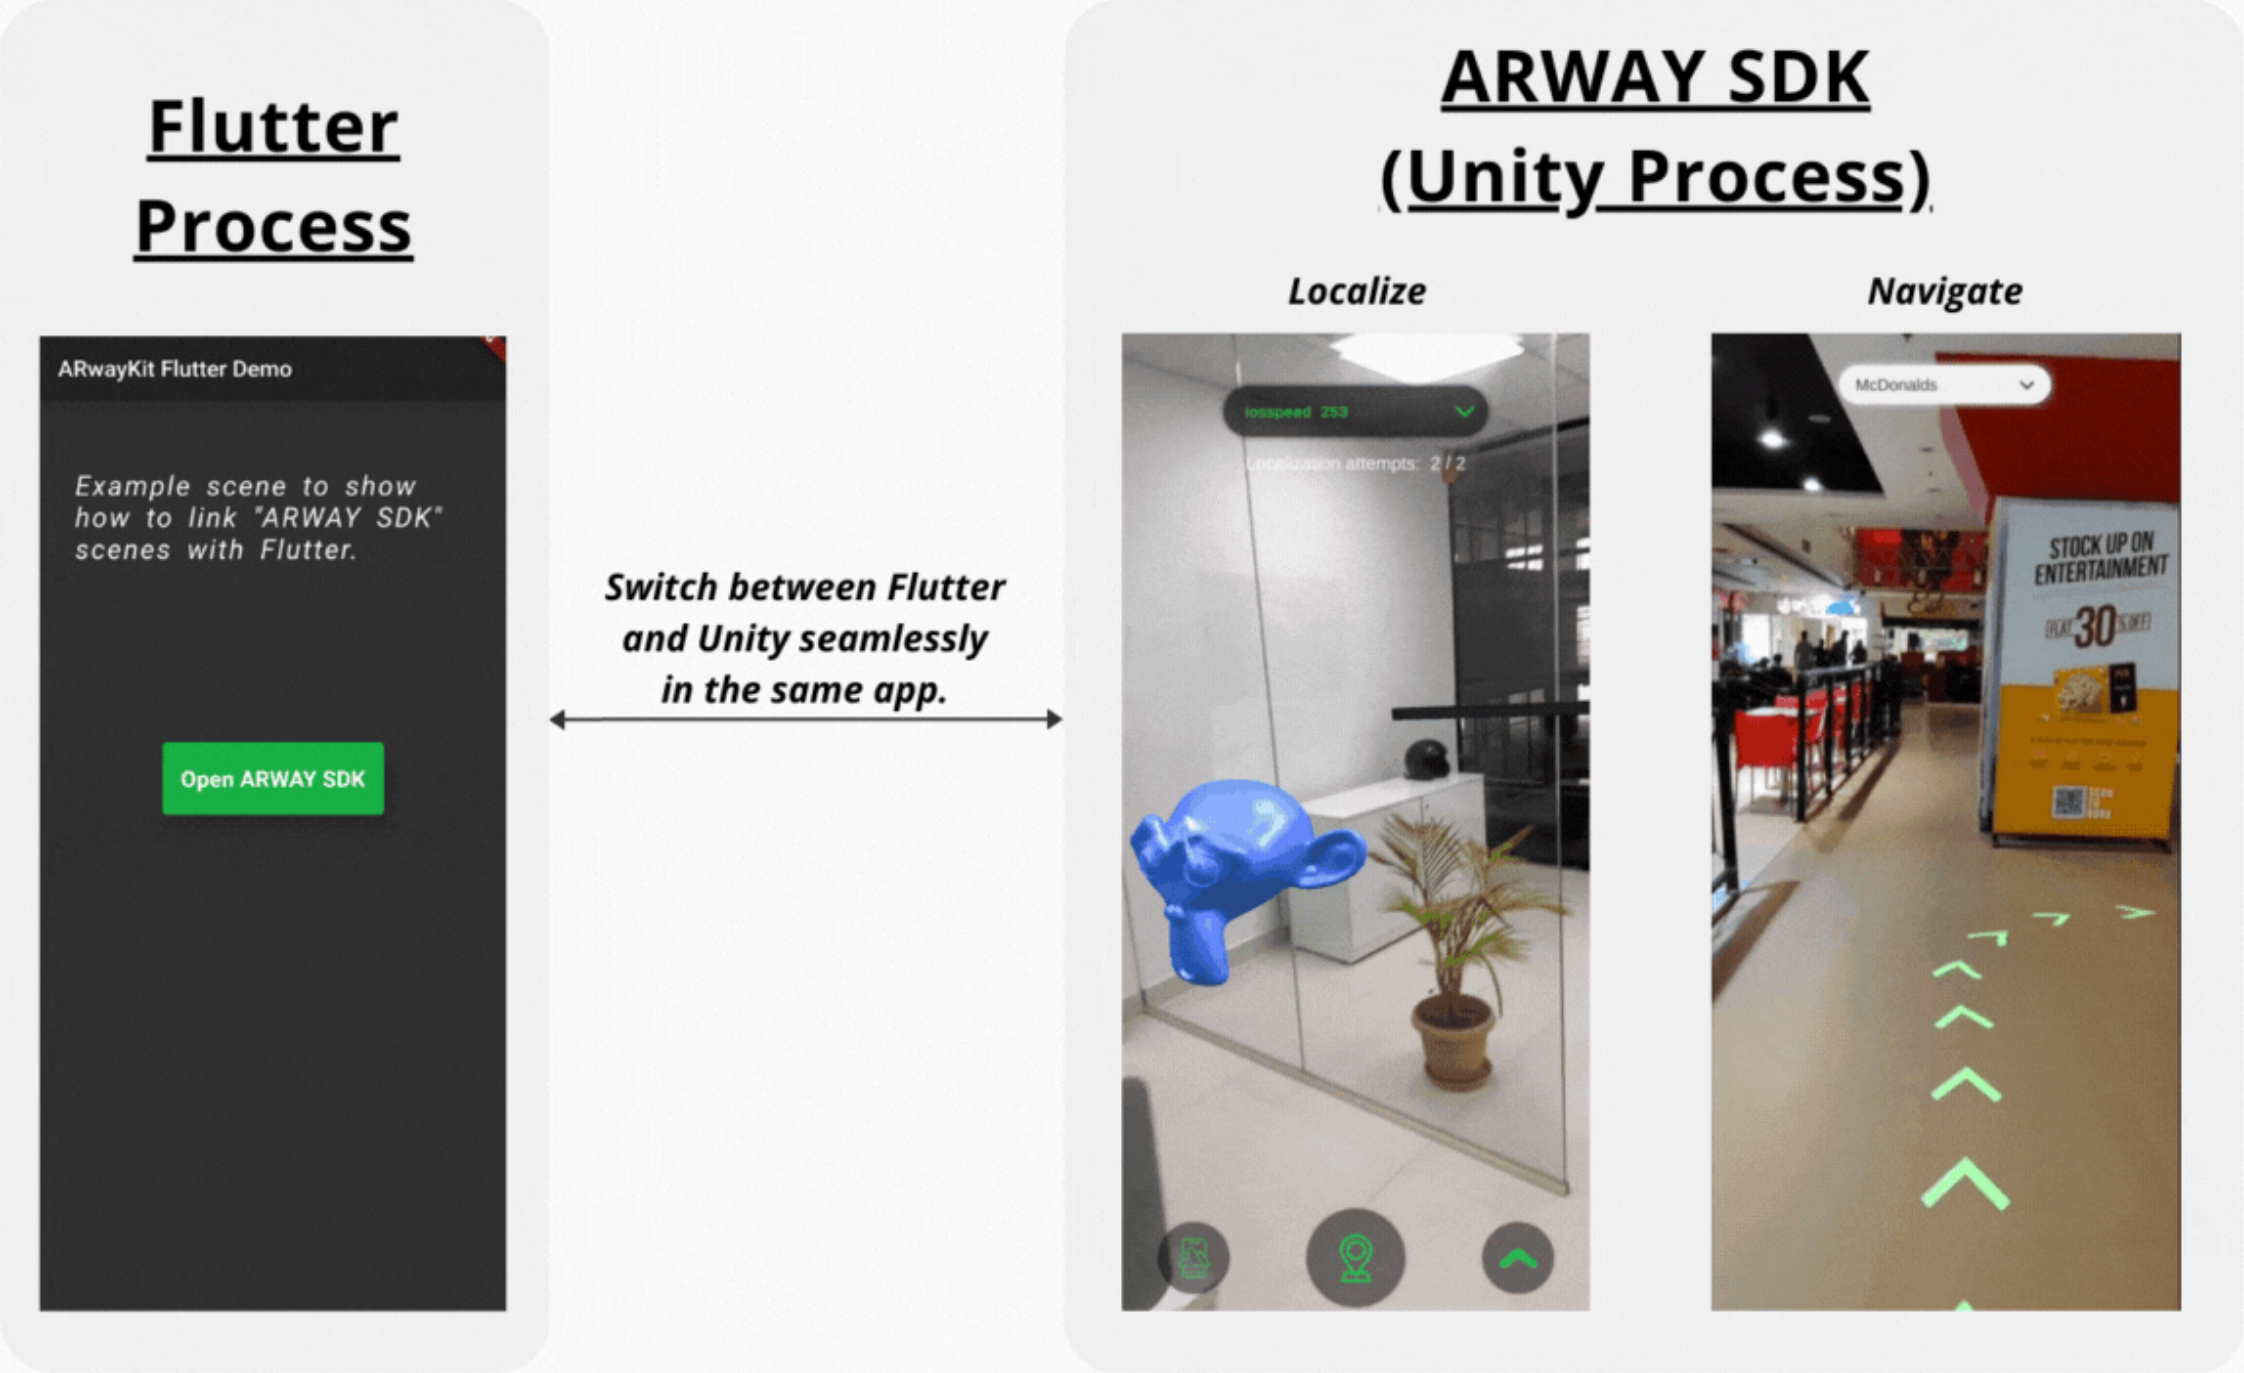
\includegraphics[width=\textwidth]{ARwayKit_samplegif_screenshot}
  \caption[Realtà aumentata con ARwayKit]{Immagine esempio di utilizzo realtà aumentata con ARwayKit\footnotemark}
\end{figure}
\footnotetext{Fonte: \url{https://medium.com/arway/building-ar-navigation-apps-with-flutter-and-arwaykit-280b69401cd9}}

Tuttavia, presenta delle criticità: in primo luogo obbliga l'uso di Unity (sfruttando la sua caratteristica peculiare di poter essere importato come fosse una libreria) per sviluppare la vista in realtà aumentata, il che comporta non solo dover imparare il linguaggio ma dover anche configurare ulteriori componenti (come ad esempio Unity Hub) che poi devono essere adottati assieme a quelli già in uso, appesantendo quindi il processo di codifica.\\
In secondo luogo troviamo invece il problema maggiore: la vista verrebbe realizzata nativamente in Unity, ovvero si tratta di una componente Unity separata rispetto all'applicazione che la lancia.
Questo renderebbe complesso se non impossibile usare dentro essa delle funzionalità Flutter: ad esempio, un bottone a schermo sarebbe un pulsante Unity, non Flutter, obbligando quindi poi a costruire una mappatura tra i due linguaggi per ogni funzionalità visualizzata.\\ 
Una vista così costruita non solo è scomoda da programmare, ma anche difficile da manutenere.

\subsubsection{ar\_flutter\_plugin}
\aplug{} è un \textit{plugin open-source} collaborativo estremamente giovane (il primo \textit{commit} sulla \textit{repository} pubblica risale al 6 febbraio 2021\footnote{Fonte: \url{https://github.com/CariusLars/ar_flutter_plugin/commit/da9ab148219d833755ef7a9b1e3536a3cae865d1}}) che si pone l'obiettivo di implementare componenti in realtà aumentata in Flutter.\\
Per raggiungere lo scopo si serve della libreria archiviata Sceneform\footnote{Fonte: \url{https://developers.google.com/sceneform/develop}}, che si occupa di "renderizzare scene tridimensionali realistiche in applicazioni in realtà aumentata o meno, senza dover imparare OpenGL".\\
L'architettura di \aplug{} è composta da due componenti: una \api{} multipiattaforma unificata che fornisce un'interfaccia alle applicazioni tramite il \textit{plugin} e le implementazioni specifiche per le piattaforme Android (in Kotlin) e iOS (in Swift) costruite su ARCore e ARKit rispettivamente, così da garantire accesso continuativo nel tempo a funzionalità aggiornate.\\
\aplug{} espone dei \textit{widget} che possono essere inclusi nel \textit{widget tree} (fig. \ref{fig:flutter-trees}) dell'applicazione cliente e delle classi \textit{manager} per gestire funzionalità e logiche di controllo del \textit{plugin} e delle componenti in realtà aumentata: il \textit{session manager} gestisce le configurazioni di tracciamento (ad esempio se gestire piani orizzontali, verticali o entrambi), opzioni di \textit{debugging} (come la visualizzazione dei piani) e le \textit{callbacks} per gli \textit{hit-test}\footnote{Immaginando un vettore che parte dall'ottica del dispositivo e tocca una superficie, possiamo considerare quel contatto un \textit{"hit"}. Con \textit{hit-testing} si intende valutare la capacità di tracciare correttamente lo spazio inteso come distanza tra i punti dello stesso e il dispositivo.} e i \textit{gesture events}\footnote{Azioni che il sistema deve fare quando vengono effettuati degli \textit{input} tramite \textit{touch screen} del dispositivo}.\\
L'\textit{object manager} gestisce i nodi in realtà aumentata del \textit{plugin} che servono ad astrarre rispetto alle funzionalità native delle varie piattaforme (ARCore e ARKit ad esempio) e permettono di aggiungere, modificare o rimuovere nodi basandosi su formati GLTF2 o GLB che possono essere caricati a \textit{runtime} da un \textit{file system} o dalla rete.\\
L'\textit{anchor manager} contiene funzioni per caricare e ottenere ancoraggi da servizi \textit{cloud} servendosi della \api{} Google Coud Anchor. Gli ambienti virtuali registrati localmente possono essere salvati in rete e comparati con quelli già in \textit{storage} persistente per scaricare ancoraggi e oggetti precedentemente posizionati nella scena.\\
Infine il \textit{location manager} si occupa di fornire le coordinate del \textit{global positioning system}  per permettere un'interrogazione efficiente degli ancoraggi basati su posizione geografica.\\
Il \textit{plugin} ha un'architettura largamente \textit{clout-agnostic}, ovvero che non si interessa dell'implementazione specifica per i servizi di salvataggio persistente, il che gli permette di usare facilmente gestori di contenuti esterni.

\subsubsection{Confronto}
Vediamo quindi di schematizzare e mettere a confronto pregi e difetti delle due soluzioni trovate.\aCapo{}

\textbf{Pregi ARwayKit:}
\begin{itemize}
  \item Implementa nativamente le \asa{};
  \item Funziona in ambienti \textit{GPS-denied};
  \item E' pensato per uso aziendale.
\end{itemize}

\textbf{Difetti ARwayKit:}
\begin{itemize}
  \item La vista e le componenti in realtà aumentata non sono implementate in Flutter;
  \item Richiede l'uso di Unity che, essendo un motore per videogiochi, ha funzionalità in più (e in meno) non necessarie (e necessarie) rispetto a un uso aziendale;
  \item Ha una documentazione difficile da reperire e di dubbia completezza;
  \item E' codice propietario, quindi non c'è modo di visionare il sorgente.
\end{itemize}

\textbf{Pregi \aplug{}:}
\begin{itemize}
  \item La vista e le componenti in realtà aumentata sono implementate in Flutter;
  \item Ha un documentazione discreta;
  \item E' \textit{open-source}, quindi al bisogno è possibile visionare il codice sorgente;
  \item E' pensato per uso aziendale;
  \item La struttura logica, divisa nei vari \textit{manager}, è modulare e chiara da comprendere, il che dovrebbe facilitarne modifica ed estensione;
  \item Promette di essere \textit{cloud-agnostic}, quindi favorisce l'uso di gestorie sterni come ad esempio \asa{} 
\end{itemize}

\textbf{Difetti \aplug{}:}
\begin{itemize}
  \item Non implementa nativamente le \asa{}, usando invece le Google Cloud Anchors;
  \item Non è chiaro se funzioni nativamente in ambienti \textit{GPS-denied};
\end{itemize}

\textbf{Confronto schematico:}

{
  \setlength{\freewidth}{\dimexpr\textwidth-10\tabcolsep}
  \renewcommand{\arraystretch}{1.5}
  \centering
  \setlength{\aboverulesep}{0pt}
  \setlength{\belowrulesep}{0pt}
  \begin{longtable}{C{.6\freewidth} C{.2\freewidth} C{.2\freewidth}} 
     \toprule 
  \cellcolor{red}\textcolor{white}{\textbf{Caratteristica}} &
  \cellcolor{red}\textcolor{white}{\textbf{ARwayKit}} &
  \cellcolor{red}\textcolor{white}{\textbf{Plugin}}\\
  \midrule
  \endhead
  
  \cellcolor{black!20}\asa{} native & \cellcolor{green!20}SI & \cellcolor{red!20}NO\\
  \cellcolor{black!20}Ambienti \textit{GPS-denied} & \cellcolor{green!20}SI & \cellcolor{orange!20}NON CHIARO\\
  \cellcolor{black!20}Vista realtà aumentata implementata in Flutter & \cellcolor{red!20}NO & \cellcolor{green!20}SI\\
  \cellcolor{black!20}Codice sorgente visibile & \cellcolor{red!20}NO & \cellcolor{green!20}SI\\
  \cellcolor{black!20}Pensato per uso aziendale & \cellcolor{green!20}SI & \cellcolor{green!20}SI\\

  \bottomrule
  \rowcolor{white} 
  \caption{Confronto \textit{framework} per realtà aumentata}
  \end{longtable}
}

E' stato infine scelto \aplug{} rispetto ad ARwayKit per evitare di interfacciarsi con Unity e per la necessità di avere la vista in realtà aumentata implementata direttamente in Flutter.

\section{Analisi dei requisiti}
Di seguito sono riportati i requisti individuati nel piano di lavoro proposto e a seguito di opportuni confronti con il tutor aziendale. Essi sono catalogati secondo la dicitura:
\begin{center}
    \textbf{R[Obbligatorietà][Tipologia][Codice]}
\end{center}
dove:
\begin{itemize}
    \item \textbf{Obbligatorietà}: specifica quanto un requisito sia vincolante per la riuscita del prodotto e può assumere i seguenti valori:
    \begin{itemize}
        \item \textbf{1: } Requisito obbligatorio;
        \item \textbf{2: } Requisito desiderabile ma non essenziale per il funzionamento;
        \item \textbf{3: } Requisito opzionale.
    \end{itemize}
    \item \textbf{Tipologia}: specifica la tipologia del requisito e può assumere i seguenti valori:
    \begin{itemize}
        \item \textbf{F: }\textit{funzionale,} determina una funzionalità necessaria all'applicazione;
        \item \textbf{V: }\textit{vincolo,} riguarda una caratteristica del prodotto decisa a monte.
    \end{itemize}
    \item \textbf{Codice}: identifica univocamente un requisito all'interno della sua tipologia (ovvero possono esistere due requisiti con lo stesso codice a patto che siano uno funzionale e uno di vincolo). Per i requisti subordinati si usa il "punto" come divisorio (\textit{ReqPadre, ReqPadre.Figlio1})
\end{itemize}

\subsection{Requisiti funzionali}
{
    \setlength{\freewidth}{\dimexpr\textwidth-10\tabcolsep}
    \renewcommand{\arraystretch}{1.5}
    \centering
    \setlength{\aboverulesep}{0pt}
    \setlength{\belowrulesep}{0pt}
    \rowcolors{2}{red!10}{white}
    \begin{longtable}{C{.15\freewidth} C{1\freewidth}}
       \toprule
    \rowcolor{red}
    \textcolor{white}{\textbf{Codice}}&
    \textcolor{white}{\textbf{Descrizione}}\\
    \toprule
    \endhead

    R1F1 & Il \textit{plugin} deve rappresentare \textit{asset} tramite ancoraggio in realtà aumentata\\
    R1F2 & Il \textit{plugin} deve rappresentare \textit{ticket} tramite ancoraggio in realtà aumentata\\
    R1F3 & Il \textit{plugin} deve integrare gli ancoraggi tramite \asa{}\\
    R1F3.1 & Permettere aggiunta di \asa\\%C
    R1F3.2 & Permettere recupero e visualizzazione di \asa\\%R
    R2F3.3 & Permettere modifica di \asa\\%U
    R1F3.4 & Permettere eliminazione di \asa\\%D
    %API BACKEND
    R1F4 & Comunicare con le \api{}s di Syn\\
    R1F4.1 & Ricevere \textit{asset} con ancoraggio associato\\
    R1F4.2 & Aggiungere \textit{asset} con ancoraggio associato\\
    R2F4.3 & Ricevere \textit{ticket} con ancoraggio associato\\
    R2F4.4 & Aggiungere \textit{ticket} con ancoraggio associato\\
    %UI FLUTTER
    R1F5 & Utente deve poter vedere quali \textit{asset} hanno ancoraggio associato\\
    R2F6 & Utente deve poter vedere quali \textit{ticket} hanno ancoraggio associato\\
    R1F7 & Utente deve poter raggiungere l'ancoraggio in vista in realtà aumentata dalla schermata dell'\textit{asset}\\
    R1F8 & \textit{On-Tap} su una ancoraggio deve aprire una \textit{bottom sheet} contestuale\\
    R1F8.1 & \textit{Bottom sheet} deve presentare identificatore per \textit{asset} o \textit{ticket} associato all'ancoraggio\\
    R1F8.2 & \textit{Bottom sheet} associato a un \textit{asset} mostra ultimi tre \textit{ticket} aperti\\
    R1F8.3 & \textit{Bottom sheet} deve fornire \textit{Call-To-Action} per eliminare l'ancoraggio\\
    R1F8.4 & \textit{Bottom sheet} deve fornire \textit{Call-To-Action} per raggiungere pagina di dettaglio\\
    R1F9 & Le informazioni contestuali di un \textit{ticket} includono data e ora di creazione\\
    %UI AR
    R1F10 & Gli ancoraggi hanno rappresentazione visiva contestuale\\ 
    R1F11 & \textit{On-Tap} sullo spazio permette di creare una ancoraggio in posizione\\
    R1F11.1 & Ancoraggio posizionato nello spazio può essere salvato\\
    R1F11.2 & Ancoraggio posizionato nello spazio può essere eliminato\\
    R1F12 & Il salvataggio di un'ancoraggio è disponibile solo quando è sicuro vada a buon fine\\
    R1F12.1 & Viene mostrato a schermo un feedback riguardo il livello di sicurezza raggiunto\\
    \bottomrule
    \rowcolor{white} 
    \caption{Tabella dei requisiti funzionali}
    \label{tab:requisiti-funzionali}
    \end{longtable}
}

\subsection{Requisiti di vincolo}
{
    \setlength{\freewidth}{\dimexpr\textwidth-10\tabcolsep}
    \renewcommand{\arraystretch}{1.5}
    \centering
    \setlength{\aboverulesep}{0pt}
    \setlength{\belowrulesep}{0pt}
    \rowcolors{2}{red!10}{white}
    \begin{longtable}{C{.15\freewidth} C{1\freewidth}} 
       \toprule
    \rowcolor{red}
    \textcolor{white}{\textbf{Codice}}&
    \textcolor{white}{\textbf{Descrizione}}\\
    \toprule
    \endhead

    R1V1 & \textit{Framework} scelto funziona su Android\\
    R2V2 & \textit{Framework} scelto funziona su iOS\\
    R1V3 & \textit{Framework} scelto si integra con le \api{}s di Syn\\
    R1V3.1 & \textit{Framework} ottiene con ancoraggio associato i dati degli \textit{asset}\\
    R1V3.2 & \textit{Framework} ottiene con ancoraggio associato i dati dei \textit{ticket}\\
    R1V4 & Il \textit{framework} scelto utilizza \asa\\
    R1V5 & La vista in realtà aumentata deve essere sviluppata in Flutter\\
    \bottomrule
    \rowcolor{white} 
    \caption{Tabella dei requisiti di vincolo}
    \label{tab:requisiti-di-vincolo}
    \end{longtable}
}

\subsection{Riepilogo requisiti}
Sono stati individuati un totale di 36 requisiti, 29 funzionali e 7 di vincolo, di seguito schematizzati:
{
    \setlength{\freewidth}{\dimexpr\textwidth-10\tabcolsep}
    \renewcommand{\arraystretch}{1.5}
    \centering
    \setlength{\aboverulesep}{0pt}
    \setlength{\belowrulesep}{0pt}
    \rowcolors{2}{red!10}{white}
    \begin{longtable}{C{.25\freewidth} C{.2\freewidth}} 
       \toprule
    \rowcolor{red}
    \textcolor{white}{\textbf{Obbligatorietà}}&
    \textcolor{white}{\textbf{Quantità}}\\
    \toprule
    \endhead

    Obbligatori & 31\\
    Desiderabili & 5\\
    \bottomrule
    \rowcolor{white} 
    \caption{Numero di requisiti per obbligatorietà}
    \label{tab:requisiti-obbligatorieta}
    \end{longtable}
}

{
    \setlength{\freewidth}{\dimexpr\textwidth-10\tabcolsep}
    \renewcommand{\arraystretch}{1.5}
    \centering
    \setlength{\aboverulesep}{0pt}
    \setlength{\belowrulesep}{0pt}
    \rowcolors{2}{red!10}{white}
    \begin{longtable}{C{.25\freewidth} C{.2\freewidth}} 
       \toprule
    \rowcolor{red}
    \textcolor{white}{\textbf{Tipologia}}&
    \textcolor{white}{\textbf{Quantità}}\\
    \toprule
    \endhead

    Funzionali & 29\\
    Di Vincolo & 7\\
    \bottomrule
    \rowcolor{white} 
    \caption{Numero di requisiti per tipologia}
    \label{tab:requisiti-tipolgia}
    \end{longtable}
}


%************************************************************************************************************

\section{Pianificazione}
\label{sec:pianificazione}
La natura estremamente sperimentale di questo progetto ha reso vano ogni tentativo di pianificare accuratamente il lavoro (complici anche le problematiche che vedremo nella sezione \ref{sec:difficolta_incontrate}).\\
Per questo motivo, una volta scelto il \textit{framework} per l'implementazione di \asa{} in Flutter l'approccio scelto è stato di \textit{trial-and-error}, e ha impegnato una buona parte del tempo di stage sia mio che dei membri di Datasoil responsabili del \textit{frontend}.\\
E' stata comunque fatta, di settimana in settimana, una scaletta degli obiettivi da raggiungere per il lunedì successivo, tuttavia si è riusciti a seguirla solo fintanto che comprendeva lo studio delle tecnologie e la creazione di brevi \textit{proof of concept} (ad esempio costruire un'applicazione in Dart e poi tradurre i suoi \textit{stateful widget} in \textit{hook widget}).\\
Riporto quindi la programmazione settimanale che, siccome questo documento è scritto al termine dei lavori, è in parte anche un rendicontazione:

\begin{itemize}
  \item \textbf{Settimana 1:} 
      \begin{itemize}
          \item Installazione e configurazione del \textit{framework} Flutter e della \sdk{} per Android 
          \item Configurazione emulatore Android (scelto Pixel 6 API 33) e 
          \textit{developers options} sul mio telefono personale;
          \item Configurazione \vsc{} e \astudio;
          \item Sviluppo di applicazione d'esempio con Flutter che sfrutta gli \textit{stateful widgets};
      \end{itemize} 
  \item \textbf{Settimana 2:} 
      \begin{itemize}
          \item Studio degli \textit{hook widgets};
          \item Traduzione degli \textit{stateful widgets} dell'applicazione d'esempio in \textit{hook widgets};
          \item Sviluppo applicazione d'esempio con gli \textit{hook widgets};
      \end{itemize}
  \item \textbf{Settimana 3:} 
      \begin{itemize}
          \item Studio delle \asa;
          \item Creazione risorse necessarie nel portale di Azure;
          \item Sviluppo applicazione di esempio per \asa{};
      \end{itemize}
  \item \textbf{Settimana 4:} Studio dei metodi per implementare le asa in Flutter:
      \begin{itemize}
          \item Studio dei \textit{method channels};
          \item Studio di ARwayKit e valutazione del suo approccio tramite Unity;
          \item Studio di \aplug;
      \end{itemize}
  \item \textbf{Settimana 5:} 
      \begin{itemize}
          \item Adattamento dell'esempio \aplug{} per integrarci le \asa{};
          \item Lettura dei \textit{logs} per filtrarne gli \textit{output};
      \end{itemize}
  \item \textbf{Settimana 6:} 
      \begin{itemize}
        \item Utilizzo diretto di ARCore in Flutter per capirne il flusso;
        \item Integrazione \asa{} in Flutter;
      \end{itemize}
  \item \textbf{Settimana 7:} Integrazione componenti realtà aumentata in MobileSYN lato Android;
  \item \textbf{Settimana 8:} Integrazione componenti realtà aumentata in MobileSYN lato iOS;
\end{itemize}

I processi di verifica e validazione non hanno potuto fare affidamento su sistemi consolidati, in quanto tutto il lavoro è stato genuinamente sperimentale, e quindi ci si è affidati al \textit{testing} "sul campo", ovvero provando direttamente l'applicazione (a un certo punto usando direttamente la versione in produzione) per valutare il progresso dei lavori e scoprire la presenza o meno di errori.\\
Di grande aiuto sono stati i \textit{logs} delle varie applicazioni provate (da MobileSYN, all'applicazione di esempio di \aplug{} fino a quella di \asa{}) che hanno, in parte, sopperito alle gravi mancanze documentali delle tecnologie trattate.

%************************************************************************************************************

\section{Difficoltà incontrate}
\label{sec:difficolta_incontrate}
Le prime difficoltà incontrate a livello personale sono state di tipo tecnologico: mi sono trovato per la prima volta a dover programmare con linguaggi orientati al \textit{frontend}, dovendo quindi cambiare almeno in parte il mio \textit{modus operandi} nella progettazione e scrittura di codice. A questo si è aggiunta la necessità di gestire altri tre linguaggi per le implementazioni native, ovvero Java e Kotlin per il lato Android e Swift per la parte iOS e, a complicare le cose, tutti questi linguaggi dovevano essere messi in comunicazione diretta con Flutter (e nel caso di Java e Kotlin anche tra di loro).\\ 
Una buona parte dello \textit{stage} è quindi stata investita nel comprendere e nel gestire la grande diversità di linguaggi diversi.\\
In linea più generale invece le due problematiche che hanno più di tutte complicato i lavori (sia per me che per Datasoil stessa) sono stati la mancanza di documentazione adeguata e di supporto da parte della comunità degli sviluppatori.\\
Microsoft non fornisce un supporto documentale adeguato per quanto riguarda \asa{}, mostrando il meno possibile della struttura interna (ad esempio come viene rappresentato un ancoraggio) e fornendo solo \api{} per effettuare operazioni ad alto livello (come il salvataggio in \textit{cloud} di un'\textit{anchor}), inoltre la ricerca della documentazione è macchinosa e richiede tempo considerevole per produrre i risultati sperati.\\
L'altro problema risiede nella difficoltà estrema di trovare supporto di terze parti (ad esempio in siti come \url{https://stackoverflow.com}), come possono dimostrare i seguenti screenshot:

\begin{figure}[H]
  \centering
  %\includegraphics[height=5cm]{screen_mobilesyn}
  
\includegraphics[width=.5\textwidth]{asa_google_search}\hfill
  
\includegraphics[width=.5\textwidth]{flutter_google_search}\\
  
\includegraphics[width=1\textwidth]{asa_flutter_google_search}
  \caption[Ricerca esatta Flutter e ASA 23 novembre]{Al 23 novembre 2022, una ricerca esatta di "flutter" mostra 87.5 milioni di risultati rilevanti, di "azure spatial anchors" 41 milioni mentre la combinazione delle due, solo 17}
\end{figure}

E a oggi (8 febbraio 2023 al momento della scrittura) la situazione non è migliorata:

\begin{figure}[H]
  \centering
  %\includegraphics[height=5cm]{screen_mobilesyn}
  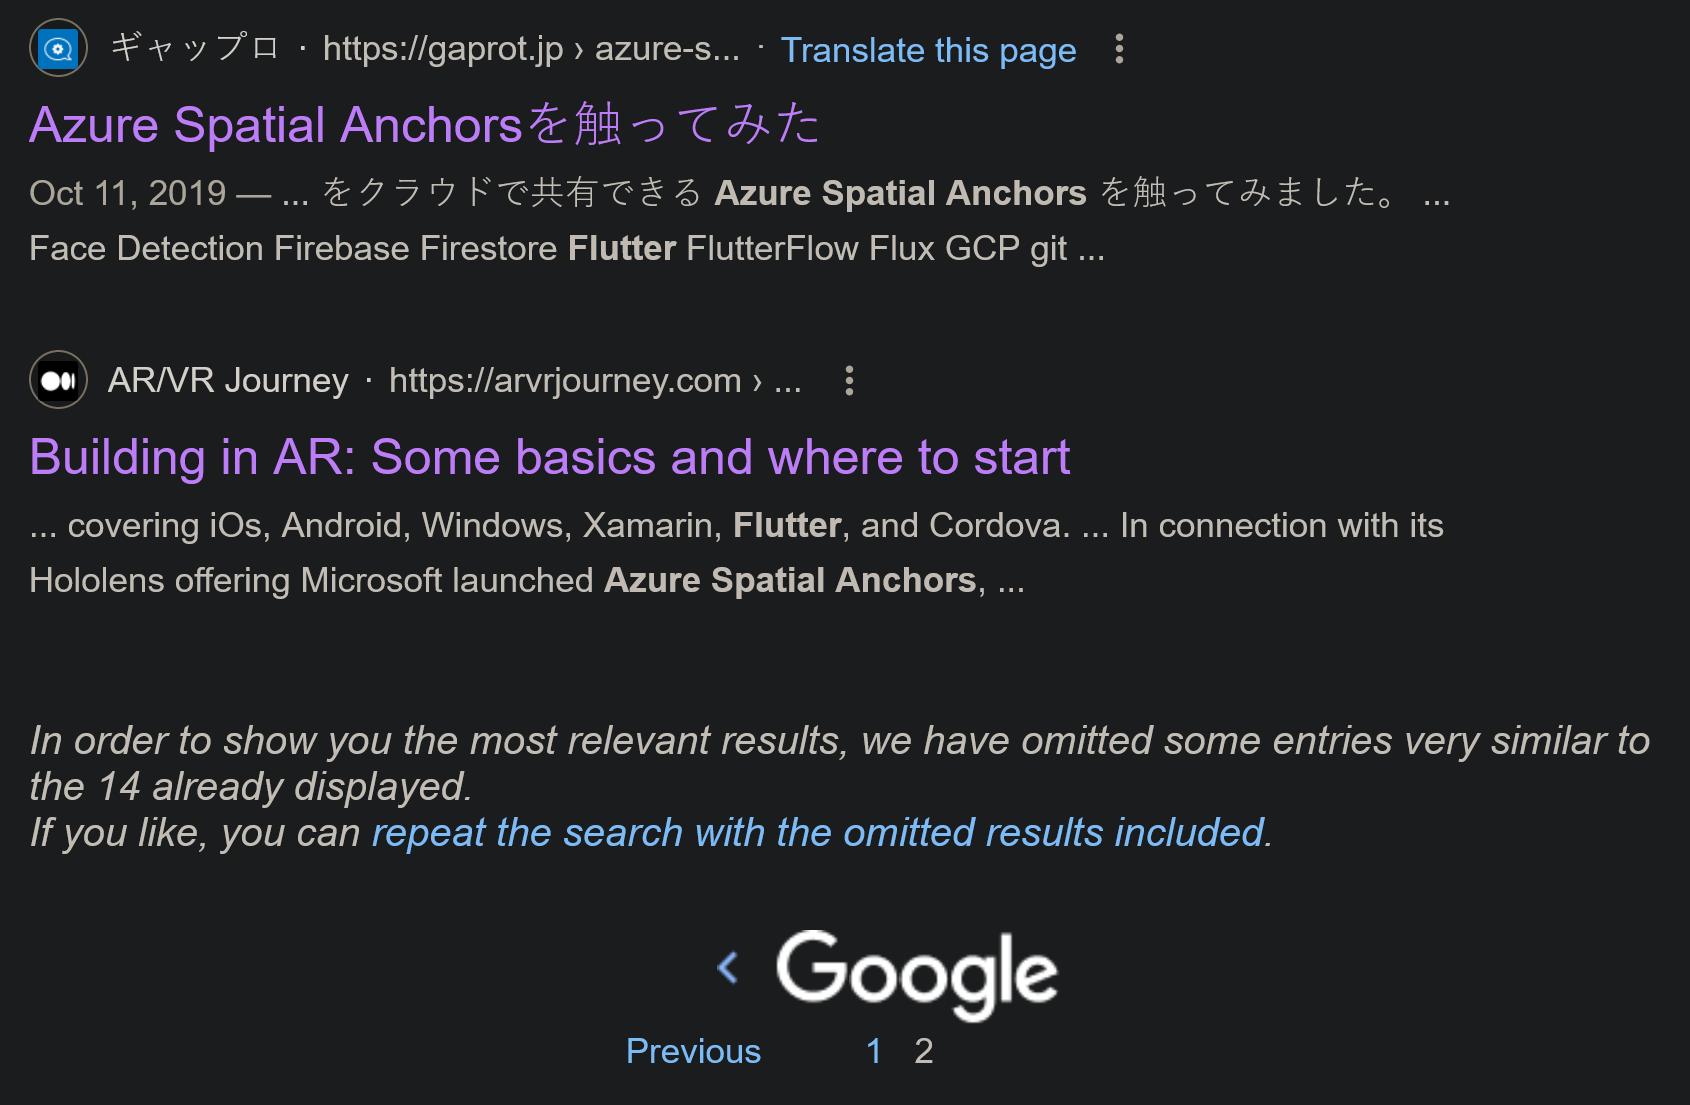
\includegraphics[width=.8\textwidth]{asa_flutter_search_today}
  \caption[Ricerca esatta Flutter e ASA 8 febbraio]{Solo 14 risultati rilevanti, alcuni in lingua giapponese, mostrano quando sia difficile trovare informazioni sull'argomento.}
\end{figure}

Questa situazione si è tradotta nella dover risolvere tutti i problemi incontrati senza poter fare affidamento su alcun aiuto esterno e ha quindi esacerbato ulteriormente l'approccio \textit{trial-and-error} di cui si è parlato nella sezione \ref{sec:pianificazione}.

%************************************************************************************************************

\section{Risultati raggiunti}
\subsection{Copertura requisiti}
\subsection{Implementazione Android}
\subsection{Implementazione iOS}
